\documentclass[11pt,a4paper,openany]{book}
\usepackage[T1]{fontenc}
\usepackage{lmodern,amsmath,amssymb,mathtools,bm,booktabs,array,tabularx,enumitem,fancyhdr,titlesec,microtype,multicol}
\usepackage[dvipsnames,svgnames]{xcolor}
\usepackage[most]{tcolorbox}
\usepackage{tikz,pgfplots}\pgfplotsset{compat=1.17}\usetikzlibrary{arrows.meta,calc,patterns}
\usepackage[hidelinks]{hyperref}
\usepackage[a4paper,margin=2.2cm,headheight=14pt]{geometry}
\setlength{\parindent}{0pt}\setlength{\parskip}{4pt}
\renewcommand{\arraystretch}{1.25}

\definecolor{navy}{HTML}{1F3864}\definecolor{sky}{HTML}{2E75B6}\definecolor{amber}{HTML}{E08A00}
\definecolor{forest}{HTML}{2E7D32}\definecolor{crimson}{HTML}{C62828}\definecolor{plum}{HTML}{5B2C83}
\definecolor{paper}{HTML}{F7F9FC}

% headings
\titleformat{\part}[display]{\bfseries\Huge\color{navy}}{\partname~\thepart}{10pt}{}
\titleformat{\chapter}[display]{\bfseries\huge\color{navy}}{\color{sky}\chaptertitlename~\thechapter}{6pt}{}[\vspace{-2pt}{\color{sky}\titlerule[1.2pt]}]
\titleformat{\section}{\Large\bfseries\color{navy}}{\thesection}{0.6em}{}
\titleformat{\subsection}{\large\bfseries\color{sky}}{\thesubsection}{0.6em}{}
\titlespacing*{\chapter}{0pt}{0pt}{16pt}
\pagestyle{fancy}\fancyhf{}\fancyhead[LE]{\small\color{gray}CSE 219 Formula \& Method Handbook}\fancyhead[RO]{\small\color{gray}\nouppercase{\leftmark}}
\fancyfoot[C]{\small\thepage}\renewcommand{\headrulewidth}{0.3pt}
\fancypagestyle{plain}{\fancyhf{}\fancyfoot[C]{\small\thepage}\renewcommand{\headrulewidth}{0pt}}

% boxes
\tcbset{enhanced,breakable,boxrule=0.6pt,arc=2pt,left=7pt,right=7pt,top=5pt,bottom=5pt,fonttitle=\bfseries\small,before skip=8pt,after skip=8pt}
\newtcolorbox{formula}[1][Key formulas]{colback=sky!7,colframe=sky,title={#1},coltitle=white,colbacktitle=sky}
\newtcolorbox{method}[1][Method]{colback=forest!6,colframe=forest,title={#1},coltitle=white,colbacktitle=forest}
\newtcolorbox{pitfall}[1][Traps]{colback=crimson!5,colframe=crimson,title={#1},coltitle=white,colbacktitle=crimson}
\newtcolorbox{inexam}[1][In the exam]{colback=amber!8,colframe=amber,title={#1},coltitle=white,colbacktitle=amber}
\newtcolorbox{example}[1]{colback=paper,colframe=plum,title={Worked example --- #1},coltitle=white,colbacktitle=plum}
\newtcolorbox{proofbox}[1][Proof]{colback=white,colframe=navy!70,title={#1},coltitle=white,colbacktitle=navy!70}
\newenvironment{steps}{\begin{enumerate}[leftmargin=1.6em,itemsep=1pt,topsep=2pt,label=\bfseries\color{forest}\arabic*.]}{\end{enumerate}}

% math macros
\newcommand{\jw}{j\omega}\newcommand{\Xjw}{X(j\omega)}\newcommand{\ejw}[1]{e^{#1}}
\newcommand{\E}{\mathrm{e}}\newcommand{\dd}{\,\mathrm{d}}
\newcommand{\ak}{a_k}\newcommand{\wo}{\omega_0}
\newcommand{\Z}{\mathcal{Z}}\newcommand{\Lap}{\mathcal{L}}\newcommand{\F}{\mathcal{F}}
\newcommand{\rect}{\operatorname{rect}}\newcommand{\sinc}{\operatorname{sinc}}\newcommand{\sgn}{\operatorname{sgn}}
\renewcommand{\Re}{\operatorname{Re}}
\newcommand{\ROC}{\mathrm{ROC}}
\DeclarePairedDelimiter{\abs}{\lvert}{\rvert}
\newcommand{\pair}{\;\longleftrightarrow\;}
\newcommand{\mk}[1]{{\color{crimson}\bfseries#1}}

\begin{document}
\frontmatter
\begin{titlepage}
\begin{tikzpicture}[remember picture,overlay]
\fill[navy] (current page.north west) rectangle ($(current page.north east)+(0,-9cm)$);
\fill[sky] ($(current page.north west)+(0,-9cm)$) rectangle ($(current page.north east)+(0,-9.35cm)$);
\node[anchor=north west,text=white,align=left,inner sep=0] at ($(current page.north west)+(2.2cm,-2.6cm)$) {\fontsize{34}{38}\selectfont\bfseries CSE 219\\[4pt]\fontsize{22}{26}\selectfont Signals and Linear Systems};
\node[anchor=north west,text=white!85!navy,align=left,inner sep=0] at ($(current page.north west)+(2.2cm,-6.6cm)$) {\Large Formulas, Methods and Worked Patterns\\ for the Term Final};
\end{tikzpicture}
\vspace*{10.2cm}

{\large\color{navy}\bfseries What this handbook covers}\par\smallskip
\begin{tabular}{@{}p{0.47\textwidth}p{0.47\textwidth}@{}}
\textbf{Part I --- Anik Sir} (Lectures 1--7)\newline Signals, LTI systems and convolution, Fourier series, Fourier transform. &
\textbf{Part II --- Ashraf Sir}\newline DTFT/DFT, FFT, sampling, Laplace and $z$-transform.\\
\end{tabular}
\vfill
\begin{tcolorbox}[colback=paper,colframe=navy!40]
\small Built from the lecture slides, the 2022--23 and 2023--24 CSE 219 term finals, the earlier EEE~211/301 and CSE~311 papers on the same content, and both practice sets. Every formula is stated once, followed by the \emph{general procedure} to attack that question type and a worked example taken from a past paper.
\end{tcolorbox}
\end{titlepage}

\chapter*{How to Use This Handbook}
\addcontentsline{toc}{chapter}{How to Use This Handbook}
\begin{tabularx}{\textwidth}{@{}>{\bfseries}p{2.6cm}X@{}}
\textcolor{sky}{Blue box} & The formulas to know by heart.\\
\textcolor{forest}{Green box} & The step-by-step procedure for a question type.\\
\textcolor{crimson}{Red box} & Common traps and sign/limit mistakes.\\
\textcolor{amber}{Amber box} & Which TF questions this appears in, and what they ask.\\
\textcolor{plum}{Purple box} & A fully worked example from a past paper or the practice sets.\\
\end{tabularx}

\medskip
\textbf{Scope notes.} Anik Sir's syllabus excludes slides marked $(*)$ and Parseval's theorem; long foundation derivations are for intuition only. Short proofs are given in compact form (see the \emph{Proofs} boxes). Ashraf Sir's Lecture~0 is history and not examinable.

\tableofcontents

\mainmatter
\part{Foundations --- the Basics You Need First}

%=====================================================================
\chapter{Mathematical Basics for Signals and Systems}
%=====================================================================
Every method in this handbook rests on a short list of tools. If a step in a later solution feels like a ``trick'', it is almost certainly one of the items below.

\section{Complex numbers and Euler's formula}
\begin{formula}
\begin{align*}
z&=a+jb=re^{j\theta},\qquad r=\abs z=\sqrt{a^2+b^2},\ \ \theta=\operatorname{atan2}(b,a),\qquad j^2=-1,\\
e^{j\theta}&=\cos\theta+j\sin\theta,\qquad \cos\theta=\frac{e^{j\theta}+e^{-j\theta}}2,\qquad \sin\theta=\frac{e^{j\theta}-e^{-j\theta}}{2j},\\
z^*&=a-jb=re^{-j\theta},\qquad zz^*=\abs z^2,\qquad \frac1z=\frac{z^*}{\abs z^2},\\
\abs{z_1z_2}&=\abs{z_1}\abs{z_2},\quad \angle(z_1z_2)=\angle z_1+\angle z_2,\qquad \operatorname{Re}z=\frac{z+z^*}2,\ \ \operatorname{Im}z=\frac{z-z^*}{2j}.
\end{align*}
\end{formula}
\begin{formula}[Special values to memorise]
\[e^{j0}=1,\ e^{j\pi/2}=j,\ e^{j\pi}=-1,\ e^{-j\pi/2}=-j,\ e^{j2\pi k}=1,\ e^{j\pi k}=(-1)^k,\ j=e^{j\pi/2},\ \tfrac1j=-j.\]
\[\frac{1-j}{\sqrt2}=e^{-j\pi/4},\qquad \frac{1+j}{\sqrt2}=e^{j\pi/4},\qquad \sqrt{2}\,e^{j\pi/4}=1+j.\]
\end{formula}
\begin{method}[Rectangular $\leftrightarrow$ polar]
\begin{steps}
\item Magnitude $r=\sqrt{a^2+b^2}$. Angle: look at the quadrant first (a calculator's $\tan^{-1}$ only gives $-90^\circ..90^\circ$). If $a<0$ add $\pm\pi$.
\item To \emph{multiply or divide} use polar form; to \emph{add or subtract} use rectangular form.
\item A complex number with $\theta=0$ or $\pi$ is real; $\pm\pi/2$ is purely imaginary.
\end{steps}
\end{method}
\begin{example}{amplitude and phase of a ratio}
$H(j\omega)=\dfrac1{2+j\omega}$ at $\omega=3$: $\abs H=\dfrac1{\sqrt{13}}=0.277$, $\angle H=-\tan^{-1}\frac32=-56.3^\circ$. (The phase of a ratio is $\angle\text{num}-\angle\text{den}$.)
\end{example}

\section{Trigonometric identities}
\begin{formula}
\begin{align*}
\sin^2\theta+\cos^2\theta&=1, & \cos^2\theta&=\tfrac12(1+\cos2\theta), & \sin^2\theta&=\tfrac12(1-\cos2\theta),\\
\sin2\theta&=2\sin\theta\cos\theta, & \cos(A\pm B)&=\cos A\cos B\mp\sin A\sin B, & \sin(A\pm B)&=\sin A\cos B\pm\cos A\sin B,\\
\cos A\cos B&=\tfrac12[\cos(A-B)+\cos(A+B)], & \sin A\sin B&=\tfrac12[\cos(A-B)-\cos(A+B)], & \sin A\cos B&=\tfrac12[\sin(A+B)+\sin(A-B)].
\end{align*}
\[\sin\theta=\cos(\theta-90^\circ),\qquad -\cos\theta=\cos(\theta\pm180^\circ),\qquad -\sin\theta=\cos(\theta+90^\circ).\]
\end{formula}
\begin{formula}[Combining sine and cosine of the same frequency]
\[A\cos\omega t+B\sin\omega t=R\cos(\omega t-\phi),\qquad R=\sqrt{A^2+B^2},\ \ \phi=\operatorname{atan2}(B,A).\]
Example: $3\cos2t+4\sin2t=5\cos(2t-53.13^\circ)$.
\end{formula}
\begin{pitfall}
Do not mix radians and degrees: the phase in $\cos(\omega t+\theta)$ must be in the same unit as $\omega t$. Write $30^\circ=\pi/6$ before substituting numbers into a formula that also has $\pi$.
\end{pitfall}

\section{Series and sums}
\begin{formula}
\begin{align*}
\sum_{n=0}^{N-1}r^n&=\frac{1-r^N}{1-r}\ (r\ne1),\qquad \sum_{n=0}^{\infty}r^n=\frac1{1-r}\ (\abs r<1),\qquad \sum_{n=n_0}^{\infty}r^n=\frac{r^{n_0}}{1-r},\\
\sum_{n=0}^{\infty}nr^n&=\frac r{(1-r)^2},\qquad \sum_{n=1}^N n=\frac{N(N+1)}2,\qquad \sum_{n=1}^N n^2=\frac{N(N+1)(2N+1)}6,\\
\sum_{n=0}^{N-1}e^{j2\pi kn/N}&=\begin{cases}N,&k\equiv0\pmod N\\0,&\text{otherwise}\end{cases}\qquad(\text{roots-of-unity sum: the heart of the DFT}).
\end{align*}
\end{formula}
\begin{method}[Evaluating a convolution or $z$-sum with limits]
\begin{steps}
\item Find the range of the summation index where the integrand/sequence is non-zero (draw $x[k]$ and $h[n-k]$ as step functions in $k$).
\item Pull out factors independent of $k$; what remains is a geometric sum $\sum r^k$.
\item Apply $\frac{r^{\text{first}}-r^{\text{last}+1}}{1-r}$; check at one small $n$ by hand.
\end{steps}
\end{method}
\begin{example}{limits of a geometric sum}
$\sum_{k=-\infty}^{-1}12^k=\dfrac{12^{-1}}{1-12^{-1}}=\dfrac1{11}$ (first term $12^{-1}$, ratio $\frac1{12}$ going \emph{downwards}). Always ask: ``which end of the sum converges?''
\end{example}

\section{Calculus you actually use}
\begin{formula}
\begin{align*}
\int e^{at}\dd t&=\frac{e^{at}}a,\qquad \int te^{at}\dd t=\frac{e^{at}(at-1)}{a^2},\qquad \int_0^\infty t^ne^{-at}\dd t=\frac{n!}{a^{n+1}}\ (a>0),\\
\int e^{at}\cos bt\dd t&=\frac{e^{at}(a\cos bt+b\sin bt)}{a^2+b^2},\qquad \int e^{at}\sin bt\dd t=\frac{e^{at}(a\sin bt-b\cos bt)}{a^2+b^2},\\
\int_{-\infty}^{\infty}\frac{\dd x}{a^2+x^2}&=\frac\pi a,\qquad \int_{-\infty}^\infty\frac{\sin x}{x}\dd x=\pi,\qquad \int_{-\infty}^\infty\Big(\frac{\sin x}x\Big)^2\dd x=\pi,\\
\int_a^b u\dd v&=\big[uv\big]_a^b-\int_a^b v\dd u\qquad(\text{integration by parts: choose $u$ = the polynomial}).
\end{align*}
\end{formula}
\begin{formula}[Symmetric intervals]
\[\int_{-a}^{a}f_{\text{even}}\dd t=2\int_0^af\dd t,\qquad \int_{-a}^{a}f_{\text{odd}}\dd t=0.\]
Even$\times$even = even, odd$\times$odd = even, even$\times$odd = odd. This is why even signals have only cosine/real Fourier coefficients and odd signals only sines/imaginary coefficients.
\end{formula}
\begin{method}[Limits and removable singularities]
\begin{steps}
\item $0/0$: factor and cancel, or use L'H\^opital (differentiate top and bottom). Famous limits: $\frac{\sin x}x\to1$, $\frac{1-e^{-\epsilon T}}{\epsilon}\to T$, $\frac{\sin(x)}{x}$ at $x=0$ is $1$, not $0$.
\item $\operatorname{sinc}(0)=1$ and $X(s)=\frac{1-e^{-(s+a)T}}{s+a}$ is finite at $s=-a$ (value $T$).
\end{steps}
\end{method}

\section{Partial fractions}
\begin{formula}
\[\frac{N(s)}{(s-p_1)(s-p_2)}=\frac{A_1}{s-p_1}+\frac{A_2}{s-p_2},\qquad A_i=\big[(s-p_i)X(s)\big]_{s=p_i}\quad(\text{cover-up rule}).\]
\[\text{Repeated pole }p\text{ (order }m):\ \ \frac{A_1}{s-p}+\cdots+\frac{A_m}{(s-p)^m},\ \ A_{m-r}=\frac1{r!}\frac{\dd^r}{\dd s^r}\big[(s-p)^mX(s)\big]_{s=p}.\]
\end{formula}
\begin{method}[Procedure]
\begin{steps}
\item If $\deg N\ge\deg D$, divide first (the quotient is a polynomial: $\delta(t)$ terms for Laplace, a constant/delay for $z$).
\item Factor the denominator; a quadratic with complex roots stays as $\dfrac{Bs+C}{(s+\sigma)^2+\omega^2}$.
\item Find the constants by the cover-up rule; \emph{check} by evaluating both sides at one convenient value (e.g.\ $s=0$).
\item For the $z$-transform, expand $X(z)/z$ (or write in $z^{-1}$ with unit constant term) so that each term is $\frac A{1-pz^{-1}}$.
\end{steps}
\end{method}
\begin{example}{cover-up}
$\dfrac{s+2}{(s+3)(s+4)}$: at $s=-3$, $A=\frac{-1}{1}=-1$; at $s=-4$, $B=\frac{-2}{-1}=2$. Check at $s=0$: $\frac{2}{12}=\frac{-1}3+\frac24=\frac16$, correct.
\end{example}

\section{Standard signals: definitions and conventions}
\begin{formula}
\[u(t)=\begin{cases}1,&t>0\\0,&t<0\end{cases},\qquad r(t)=tu(t),\qquad \delta(t)=\frac{\dd u}{\dd t},\quad\int\delta(t)\dd t=1,\qquad \sgn t=2u(t)-1,\]
\[\rect(t)=\begin{cases}1,&\abs t<\frac12\\0,&\text{else}\end{cases},\qquad \operatorname{tri}(t)=\max(0,\,1-\abs t),\]
\[\sinc x=\frac{\sin\pi x}{\pi x}\ \text{(normalised; used with $f$ in Hz)}\qquad\text{or}\qquad \frac{\sin x}x\ \text{(unnormalised; used with $\omega$)}.\]
\end{formula}
\begin{pitfall}
Always check which \emph{sinc} convention a question uses; the two differ by a factor of $\pi$ inside the argument, and the energy $\int\sinc^2$ is $1$ (normalised) or $\pi$ (unnormalised). Also $u[n]$ equals $1$ at $n=0$, while $u(0)$ is undefined/$\frac12$ in continuous time.
\end{pitfall}

\section{The impulse: rules of the game}
\begin{formula}
\begin{align*}
\int x(t)\delta(t-t_0)\dd t&=x(t_0)\quad(\text{sifting}), & x(t)\delta(t-t_0)&=x(t_0)\delta(t-t_0),\\
\delta(at)&=\frac1{\abs a}\delta(t), & \delta(-t)&=\delta(t),\\
x(t)*\delta(t-t_0)&=x(t-t_0), & \delta[n]&=u[n]-u[n-1],\qquad x[n]=\sum_kx[k]\delta[n-k].
\end{align*}
\end{formula}
\begin{method}[Integrals containing $\delta$]
\begin{steps}
\item Find where the argument of $\delta$ vanishes ($t_0$): is $t_0$ \emph{inside} the integration limits? If not, the integral is $0$; if it sits on a limit, the problem usually says how to treat it.
\item Replace everything else by its value at $t_0$ (and divide by $\abs a$ for $\delta(at)$).
\item If $\delta$ is multiplied by a function of $t$, use $x(t)\delta(t-t_0)=x(t_0)\delta(t-t_0)$ before integrating or transforming.
\end{steps}
\end{method}

\section{Orthogonality and the idea behind Fourier analysis}
\begin{formula}
\begin{align*}
\text{inner product: }\ \langle x,z\rangle&=\int_{t_1}^{t_2}x(t)z^*(t)\dd t,\qquad \text{orthogonal}\iff\langle x,z\rangle=0,\\
\text{projection/coefficient: }\ c&=\frac{\langle x,\phi\rangle}{\langle\phi,\phi\rangle},\qquad \text{orthonormal}\iff\langle\phi_i,\phi_j\rangle=\delta_{ij},\\
\frac1T\int_Te^{j(k-m)\omega_0t}\dd t&=\begin{cases}1,&k=m\\0,&k\ne m\end{cases}\quad\Rightarrow\quad a_k=\frac1T\int_Tx(t)e^{-jk\omega_0t}\dd t .
\end{align*}
\end{formula}
Picture: in vector algebra a coordinate is a dot product with a unit axis. Fourier analysis is the same idea with the axes $e^{jk\omega_0t}$; a signal is a point with coordinates $a_k$.

\section{Systems: what the words mean}
\begin{formula}[One-line tests]
\begin{center}\small\renewcommand{\arraystretch}{1.3}\begin{tabular}{@{}lp{9cm}@{}}\toprule
linear&$T\{a x_1+bx_2\}=aT\{x_1\}+bT\{x_2\}$ (additivity + homogeneity; zero input $\Rightarrow$ zero output)\\
time-invariant&delaying the input by $t_0$ delays the output by $t_0$: $x(t-t_0)\to y(t-t_0)$\\
causal&output at $t$ depends on inputs at $\tau\le t$; for LTI, $h(t)=0$ for $t<0$\\
stable (BIBO)&bounded input $\Rightarrow$ bounded output; for LTI, $\int\abs{h}\dd t<\infty$ ($\sum\abs{h[n]}<\infty$)\\
memoryless&output at $t$ depends only on $x(t)$; for LTI, $h=K\delta(t)$\\
invertible&distinct inputs give distinct outputs\\\bottomrule\end{tabular}\end{center}
\end{formula}
\begin{formula}[LTI systems: three equivalent descriptions]
\[y=x*h\ \ \longleftrightarrow\ \ Y(\omega)=X(\omega)H(\omega)\ \ \longleftrightarrow\ \ Y(s)=X(s)H(s)\ (Y(z)=X(z)H(z)).\]
Complex exponentials are eigenfunctions: $e^{j\omega t}\to H(j\omega)e^{j\omega t}$. Cascade: $h_1*h_2$ ($H_1H_2$); parallel: $h_1+h_2$; feedback: $\frac{G}{1+GH}$.
\end{formula}

\section{Energy, power, periodicity in one glance}
\begin{formula}
\begin{align*}
E&=\int\abs{x}^2\dd t\ \ \Big(\sum\abs{x[n]}^2\Big),\qquad P=\lim\frac1{2T}\int_{-T}^{T}\abs x^2\dd t,\\
\text{periodic }T_0\ \Rightarrow\ P&=\frac1{T_0}\int_{T_0}\abs x^2\dd t\ \ (E=\infty),\qquad \text{sinusoid }A\cos(\omega t+\theta):\ P=\frac{A^2}2,\\
\text{sum of sinusoids of distinct }\omega:\ P&=\sum\frac{A_k^2}2\ \ (\text{powers add}),\qquad \text{DC }c:\ P=c^2 .
\end{align*}
\end{formula}
\begin{method}[Periodicity test]
\begin{steps}
\item Continuous time: $\cos(\omega_0t)$ has $T_0=2\pi/\omega_0$; a sum is periodic iff all ratios $\omega_i/\omega_j$ are rational; $T=$ lcm of the periods ($\omega_0=\gcd$ of the frequencies).
\item Discrete time: $e^{j\omega_0n}$ is periodic iff $\omega_0/2\pi=m/N$ is rational; $N_0=N/\gcd(m,N)$.
\end{steps}
\end{method}

\section{Logarithms, decibels and units}
\begin{formula}
\[\text{dB}=20\log_{10}\abs{H}=10\log_{10}\abs H^2,\qquad -3\text{ dB}\iff\abs H=\tfrac1{\sqrt2}\iff\text{half power},\qquad \omega=2\pi f,\ \ T=\frac1f .\]
\[e^{-1}=0.368,\ \ e^{-2}=0.135,\ \ \ln2=0.693,\ \ \pi=3.1416,\ \ \sqrt2=1.4142,\ \ \sqrt3=1.7321 .\]
\end{formula}

\section{Which transform for which problem?}
\begin{center}\small\renewcommand{\arraystretch}{1.3}\begin{tabular}{@{}p{3.6cm}p{5.4cm}p{5.2cm}@{}}\toprule
signal type&tool&use for\\\midrule
periodic, continuous&Fourier series $a_k$, $\omega_0=2\pi/T$&line spectra, power, response through a filter ($a_kH(jk\omega_0)$)\\
aperiodic, continuous&Fourier transform $X(\omega)$&bandwidth, modulation, energy, filtering\\
finite, discrete&DFT / FFT&numerical spectra, fast circular/linear convolution\\
discrete, any&DTFT, $z$-transform&frequency response, difference equations, stability\\
continuous with initial conditions&Laplace transform&circuits, ODEs, feedback and stability\\\bottomrule\end{tabular}\end{center}

\part{Anik Sir --- Signals, Systems, Fourier Series and Transform}

%=====================================================================
\chapter{Signals: Energy, Transformations, Even--Odd, Impulses, Periodicity}
%=====================================================================
\section{Energy and power}
\begin{formula}
\begin{align*}
E_{[t_1,t_2]}&=\int_{t_1}^{t_2}\abs{x(t)}^2\dd t, & E_{[n_1,n_2]}&=\sum_{n=n_1}^{n_2}\abs{x[n]}^2,\\
P_{[t_1,t_2]}&=\frac{E}{t_2-t_1}, & P_{[n_1,n_2]}&=\frac{E}{n_2-n_1+1},\\
P_\infty&=\lim_{T\to\infty}\frac1{2T}\int_{-T}^{T}\abs{x}^2\dd t .
\end{align*}
\textbf{Energy signal:} $0<E_\infty<\infty$ (then $P_\infty=0$). \textbf{Power signal:} $0<P_\infty<\infty$ (then $E_\infty=\infty$). \textbf{Neither:} both infinite.\\
Periodic signal: $P=\frac1{T_0}\int_{T_0}\abs{x}^2\dd t$. Sinusoid $A\cos(\wo t+\varphi)$: $P=A^2/2$. Complex exponential $Ae^{j\wo t}$: $P=\abs{A}^2$.
\end{formula}
\begin{method}
\begin{steps}
\item Decide the behaviour as $t\to\pm\infty$: decaying $\Rightarrow$ try energy; periodic or settling to a level $\Rightarrow$ power; growing $\Rightarrow$ neither.
\item Energy: integrate $\abs x^2$ over the support, piece by piece.
\item Power of a signal that settles to $c_-$ and $c_+$: $P_\infty=(c_-^2+c_+^2)/2$.
\item Sum of sinusoids of different frequencies: powers add.
\end{steps}
\end{method}
\begin{example}{half-sine, $x=\sin t$ on $[0,\pi]$}
$E=\int_0^\pi\sin^2t\dd t=\pi/2$, $P_{[0,\pi]}=\tfrac12$. Repeated every $\pi$: $E_\infty=\infty$, $P=\tfrac12$; repeated every $2\pi$: $P=\tfrac14$. The signal $1$ for $\abs t\le1$, $1/\abs t$ beyond has $E=2+2\int_1^\infty t^{-2}\dd t=4$ and $P=0$.
\end{example}

\section{Time shifting, reversal and scaling}
\begin{formula}
$x(t-t_0)$: delay (right) by $t_0$. $x(t+t_0)$: advance (left). $x(-t)$: mirror. $x(\alpha t)$: compress by $\alpha>1$.\\[2pt]
\[x(t)\;\xrightarrow{\text{shift by }\beta}\;x(t+\beta)\;\xrightarrow{\text{reverse if }\alpha<0}\;\;\xrightarrow{\text{scale by }|\alpha|}\;x(\alpha t+\beta)\]
A feature of $x$ at $t=a$ appears in $x(\alpha t+\beta)$ at $\boxed{t=(a-\beta)/\alpha}$.
\end{formula}
\begin{method}
\begin{steps}
\item Write $x(t)$ piecewise with all break points and values.
\item Rewrite the argument as $\alpha t+\beta$ (expand brackets: $-2(t-1)=-2t+2$).
\item Apply shift, then reversal (only if $\alpha<0$), then scaling; \emph{name every intermediate signal}.
\item Map every break point with $t=(a-\beta)/\alpha$ and keep the same shapes between them; check one interior point.
\item A sum $x(\cdot)+x(\cdot)$: sketch each term separately, then add point by point.
\end{steps}
\end{method}
\begin{pitfall}
$x(2t+3)\neq x(2(t+3))$: a shift made \emph{after} scaling acts on $t$, not on $2t$. Vertical edges stay vertical; they only move.
\end{pitfall}
\begin{example}{CSE 219 2022--23 Q7: $x(-2t+2)$ and $x(-t/2+1)$}
$x(t)=t+1\ (-2\le t<-1)$, $1\ (-1\le t\le0)$, $1-t/2\ (0<t\le2)$.\\
$x(-2t+2)$: break points $a=-2,-1,0,2\mapsto t=2,\tfrac32,1,0$, so
$x(-2t+2)=t\ (0\le t<1),\ 1\ (1\le t\le\tfrac32),\ 3-2t\ (\tfrac32<t\le2)$.\\
$x(-t/2+1)$: $t=2(1-a)=6,4,2,-2$, so $x=\tfrac12+\tfrac t4\ (-2\le t<2),\ 1\ (2\le t\le4),\ 2-\tfrac t2\ (4<t\le6)$.
\end{example}
\begin{inexam}
2023--24 Q1(a) (15): $y(t)=x(-2(t-1))+x\!\left(\tfrac{t+2}{2}\right)$, $x=1-\abs t$: two triangles, centres $t=1$ (half-width $\tfrac12$) and $t=-2$ (half-width 2), non-overlapping. 2022--23 Q7 (23). EEE: every year.
\end{inexam}

\section{Even and odd parts}
\begin{formula}
$x_e(t)=\tfrac12[x(t)+x(-t)]$, $x_o(t)=\tfrac12[x(t)-x(-t)]$, $x=x_e+x_o$. Even$\times$even=even, odd$\times$odd=even, even$\times$odd=odd; $\int_{-a}^{a}$odd$=0$; $x_o(0)=0$.
\end{formula}
\begin{method}
\begin{steps}
\item Write $x(t)$ and $x(-t)$ piecewise; the pieces of $x(-t)$ live on the mirrored intervals.
\item Cut the axis at every break point of both and compute $\tfrac12(x\pm x(-t))$ on each piece.
\item Check: $x_e$ is mirror symmetric, $x_o$ is point symmetric; their sum returns $x$.
\end{steps}
\end{method}
\begin{example}{CSE 219 2022--23 Q5(a)}
$f=t+1\ (-2\le t\le0)$, $-\tfrac t2+1\ (0<t\le2)$. For $0<t\le2$: $f_e=\tfrac12[(1-\tfrac t2)+(1-t)]=1-\tfrac{3t}4$, $f_o=\tfrac12[(1-\tfrac t2)-(1-t)]=\tfrac t4$. Hence
$f_e=1-\tfrac34\abs t$, $f_o=\tfrac t4$ for $\abs t\le2$ (zero elsewhere).
\end{example}

\section{Step, impulse and ramp}
\begin{formula}
\begin{align*}
&\delta[n]=u[n]-u[n-1],\quad u[n]=\sum_{m=-\infty}^{n}\delta[m]=\sum_{k=0}^{\infty}\delta[n-k],\\
&\delta(t)=\frac{\dd u}{\dd t},\quad u(t)=\int_{-\infty}^{t}\delta(\tau)\dd\tau,\quad r(t)=tu(t),\\
&\text{Sifting: }\int_L^R x(t)\delta(t-a)\dd t=\begin{cases}x(a)&L<a<R\\0&\text{otherwise}\end{cases},\qquad x(t)\delta(t-a)=x(a)\delta(t-a),\\
&\delta(at+b)=\tfrac1{\abs a}\delta\!\left(t+\tfrac ba\right),\qquad \int x(t)\delta'(t-a)\dd t=-x'(a),\qquad u(ct)=u(t)\ (c>0).
\end{align*}
\end{formula}
\begin{method}[Piecewise signal $\to$ elementary signals, and its derivative]
\begin{steps}
\item Scan left to right. At each break point $a$ add (new slope $-$ old slope)$\,r(t-a)$ and (jump)$\,u(t-a)$.
\item Derivative: replace $r\to u$ and $u\to\delta$. Slopes between jumps give rectangles; each jump $J$ gives $J\delta(t-a)$.
\item Second derivative: impulses at the slope changes (and $\delta'$ at jumps).
\end{steps}
\end{method}
\begin{example}{EEE 211 2022--23 Q5(c)}
$x=5t$ on $(0,1)$, $-6$ on $(1,2)$, $5(t-2)$ on $(2,3)$. At $t=1$: slope $5\to0$, jump $5\to-6$ ($-11$); at $t=2$: jump $+6$, slope $0\to5$; at $t=3$: slope $5\to0$, jump $-5$.
\[x=5r(t)-5r(t-1)-11u(t-1)+6u(t-2)+5r(t-2)-5r(t-3)-5u(t-3),\]
\[x'=5[u(t)-u(t-1)]+5[u(t-2)-u(t-3)]-11\delta(t-1)+6\delta(t-2)-5\delta(t-3).\]
\end{example}
\begin{method}[Is $p_\epsilon(t)$ a model of $\delta(t)$?]
Check three conditions: (i) area $=1$ for every $\epsilon$; (ii) $p_\epsilon(t)\to0$ for $t\neq0$; (iii) peak $\to\infty$. $p=\frac1{\epsilon\pi\cosh(t/\epsilon)}$ and $\frac1\pi\frac{\epsilon}{t^2+\epsilon^2}$ pass; $\frac1\pi\frac{\sin\epsilon t}{t}$ fails as $\epsilon\to0$ (it is a model as $\epsilon\to\infty$).
\end{method}

\section{Periodicity}
\begin{formula}
CT: $A\cos(\wo t+\varphi)$ has $T_0=2\pi/\abs{\wo}$. A sum is periodic iff the period ratio is rational; $T=\operatorname{lcm}(T_1,T_2)$.\\
DT: $x[n]=\cos(\omega_0n+\varphi)$ is periodic iff $\dfrac{2\pi}{\omega_0}=\dfrac Nm$ is rational; fundamental period $N_0=N$ in lowest terms. The phase $\varphi$ never matters.
\end{formula}
\begin{example}{DT periodicity}
$2\cos\!\left(\tfrac{16\pi}{63}n+\tfrac\pi3\right)$: $2\pi/\omega_0=63/8\Rightarrow N_0=63$. $\cos 2n$: $2\pi/2=\pi$ irrational, not periodic. $x[n]=(3-4j)e^{j13\pi n/7}$: $2\pi/\omega_0=14/13\Rightarrow N_0=14$ for both real and imaginary parts; the phase $\theta=\tan^{-1}\frac43$ is not a multiple of $\pi/7$, so it cannot be an integer time shift.
\end{example}
\begin{pitfall}
Expand squares and products first ($\sin^2\theta=\tfrac12-\tfrac12\cos2\theta$). $\sqrt{e^{j5\pi t}}=e^{j5\pi t/2}$: halve the frequency. $\delta(\sin t)$ is a train of period $\pi$.
\end{pitfall}

%=====================================================================
\chapter{LTI Systems, Convolution, Causality and Stability}
%=====================================================================
\section{System properties}
\begin{formula}
Linear: $ax_1+bx_2\mapsto ay_1+by_2$. Time-invariant: $x(t-t_0)\mapsto y(t-t_0)$. Memoryless: $y(t)$ uses only $x(t)$. Causal: $y(t)$ uses $x(\tau),\,\tau\le t$. BIBO stable: bounded in $\Rightarrow$ bounded out. Invertible: distinct inputs $\Rightarrow$ distinct outputs.
\end{formula}
\begin{method}
\begin{steps}
\item \textbf{Linear}: zero in must give zero out; apply $ax_1+bx_2$ and compare. An added constant, $\abs x$, $x^2$, $\log x$ break it.
\item \textbf{Time-invariant}: compare $S\{x(t-t_0)\}$ with $y(t-t_0)$. Variable coefficients ($t\,x$, $t^2y$), $x(2t)$, $x(-t)$ give time-variant.
\item \textbf{Causal / memory}: list which times of $x$ enter $y(t)$ ($x(t+a)$, $x(-t)$, upper limit $>t$ are non-causal).
\item \textbf{Stable}: try $x=1$ or $x=u(t)$; counterexample, or bound $\abs y\le M B$.
\end{steps}
\end{method}
\begin{example}{EEE 211 2019--20 Q1: $y=\tfrac13\!\int x(\tau)[\delta(t-\tau)+\delta(t-\tau+t_0)+\delta(t-\tau-t_0)]\dd\tau$}
Sifting: $y=\tfrac13[x(t)+x(t+t_0)+x(t-t_0)]$, a three-point moving average. Linear, time-invariant, has memory, non-causal ($x(t+t_0)$), BIBO stable ($\abs y\le B$).
\end{example}
\begin{example}{$\dfrac{\dd y}{\dd t}+t^2y=(2t+3)x$}
Linear (first power in $x,y$, zero initial state). With input $x(t-t_0)$ the coefficients $t^2$, $2t+3$ stay while $y(t-t_0)$ satisfies $(t-t_0)^2$, $2(t-t_0)+3$ --- not equal, so \mk{time-variant}.
\end{example}

\section{Impulse response and the convolution sum}
\begin{formula}
\[y[n]=\sum_{k=-\infty}^{\infty}x[k]\,h[n-k],\qquad y(t)=\int_{-\infty}^{\infty}x(\tau)h(t-\tau)\dd\tau,\qquad x*h=h*x.\]
$x*(h_1+h_2)=x*h_1+x*h_2$; cascade $h=h_1*h_2$; parallel $h=h_1+h_2$; $x(t)*\delta(t-a)=x(t-a)$.\\
Pure delay: $h[n]=\delta[n-n_0]$. Echo: $h=u[n]$ or $\alpha^nu[n]$ (larger $\alpha$, slower fade).
\end{formula}
\begin{proofbox}[Why $y=x*h$ (intuition, 4 lines)]
$x[n]=\sum_kx[k]\delta[n-k]$. Time invariance: $\delta[n-k]\to h[n-k]$. Homogeneity: $x[k]\delta[n-k]\to x[k]h[n-k]$. Additivity: $y[n]=\sum_kx[k]h[n-k]$. CT: replace $\sum$ by $\int$ using sifting.
\end{proofbox}
\begin{formula}[Finite sequences]
Length $=L+M-1$; start index $=$ sum of start indices; $\sum y=(\sum x)(\sum h)$; coefficient of $z^n$ in $A(z)B(z)$ is $\sum_ka[k]b[n-k]$.
Example: $\{1,2,1,1\}*\{1,1,-1,2\}=\{1,3,2,2,4,1,2\}$.
\end{formula}

\section{Convolution procedures}
\begin{method}[DT convolution of infinite sequences]
\begin{steps}
\item Fix $n$; $h[n-k]$ is $h$ reflected and shifted right by $n$.
\item Write the support of $x[k]$ and of $h[n-k]$ in $k$; the overlap gives the summation limits (empty $\Rightarrow$ $y[n]=0$).
\item Split into cases of $n$ where the limits change. Sum with
\[\sum_{k=0}^{n}\alpha^k=\frac{1-\alpha^{n+1}}{1-\alpha},\qquad\sum_{k=-\infty}^{m}\beta^k=\frac{\beta^m}{1-\beta^{-1}}\ (\beta>1).\]
\item Two-sided input: split $x=x_L+x_R$, convolve each, add.
\item Check: support $=$ sum of supports, continuity of the closed form at case boundaries.
\end{steps}
\end{method}
\begin{table}[h]\centering\small
\begin{tabular}{@{}lll@{}}\toprule
Pair & Result & Source\\\midrule
$x=\{0.5,2\}$, $h=\{1,1,1\}$ & $\{0.5,2.5,2.5,2\}$ & Lec 4 Ex 2.2\\
$\alpha^nu[n]*u[n]$ & $\dfrac{1-\alpha^{n+1}}{1-\alpha}u[n]$ & Ex 2.3\\
$2^nu[-n]*u[n]$ & $2^{n+1}\ (n<0)$; $2\ (n\ge0)$ & Ex 2.5\\
$\big[(\tfrac12)^nu[n]+2^nu[-n]\big]*u[n]$ & $2^{n+1}\ (n<0)$; $4-2^{-n}\ (n\ge0)$ & Ex 2.10\\
$e^{-at}u*u$ & $\tfrac1a(1-e^{-at})u(t)$ & Ex 2.6\\
$e^tu(-t)*e^{-t}u(t)$ & $\tfrac12e^{-\abs t}$ & sl.\,48--52\\
$e^{-at}u*e^{-bt}u$ & $\dfrac{e^{-bt}-e^{-at}}{a-b}u(t)$ & textbook\\\bottomrule
\end{tabular}\end{table}
\begin{example}{CSE 219 2022--23 Q8(a), 20 marks}
$x[n]=3^nu[-n-1]+(\tfrac13)^nu[n]$, $h[n]=(\tfrac14)^nu[n+3]$; $h[n-k]\ne0$ for $k\le n+3$. Left part: $\sum_{k\le\min(-1,n+3)}3^k4^{k-n}=4^{-n}\sum12^k$. Right part: $4^{-n}\sum_{k=0}^{n+3}(\tfrac43)^k$.
\[y[n]=\begin{cases}\dfrac{256}{11}3^{\,n+4},&n\le-4,\\[6pt] 256\cdot3^{-(n+3)}-\dfrac{32}{11}4^{-n},&n\ge-3.\end{cases}\]
Check: $y[-3]=69.82$ (peak), $y[0]=6.57$.
\end{example}
\begin{method}[Graphical CT convolution --- the interval table]
\begin{steps}
\item Flip the simpler signal (usually the rectangle); write its edges as functions of $t$.
\item List the $t$-intervals where an edge of one signal passes an edge/break of the other.
\item On each interval write the limits and integrate; if $x=\rect(a,b)$ then $y(t)=H(t-a)-H(t-b)$ with $H$ the running integral of $h$.
\item Check continuity at interval ends, total support, and area $\int y=\int x\int h$.
\end{steps}
\end{method}
\begin{example}{EEE 211 2023--24 Q2(a): $x=1$ on $(1,2)$, $h=$ triangle on $(-1,1)$}
\begin{center}\small\begin{tabular}{@{}ll@{}}\toprule
interval & $y(t)$\\\midrule
$t<0$ & $0$\\ $0\le t\le1$ & $t^2/2$\\ $1\le t\le2$ & $-t^2+3t-\tfrac32$\\ $2\le t\le3$ & $(3-t)^2/2$\\ $t>3$ & $0$\\\bottomrule
\end{tabular}\end{center}
Area $=1\cdot1=1$; peak $\tfrac34$ at $t=\tfrac32$.
\end{example}
\begin{example}{2023--24 Q1(b): $(h_1+h_2)*h_3$ in DT}
$h_1=\delta[n]-\delta[n-2]$, $h_2=u[n-1]$, $h_3=\delta[n]-\delta[n-1]$. $h_2*h_3=\delta[n-1]$, so $h_{eq}=\delta[n]-\delta[n-2]+\delta[n-3]$. For $x=u[n]$: $y=u[n]-u[n-2]+u[n-3]=\{1,1,0,1,1,1,\dots\}$.
\end{example}
\begin{example}{EEE 211 2023--24 Q1(c): five-system interconnection}
Branches $h_1$, $h_2*h_3=(e^{-t}-e^{-2t})u$, $h_4=\delta$: sum $=\delta+e^{-t}u$. Then $h_{eq}=\tfrac12(e^{-t}+e^{-3t})u$; $\int\abs{h_{eq}}=\tfrac23<\infty$ (stable). $y=(\tfrac12te^{-t}+\tfrac14e^{-t}-\tfrac14e^{-3t})u$.
\end{example}

\section{Causality and stability}
\begin{formula}
Causal $\Leftrightarrow h(t)=0$ for $t<0$ ($h[n]=0$, $n<0$). Stable $\Leftrightarrow\int\abs{h}\dd t<\infty$ ($\sum\abs{h[n]}<\infty$). A nonzero periodic $h$ is neither causal nor stable.
\end{formula}
\begin{proofbox}[Stability, 3 lines]
For $\abs x\le B$: $\abs{y(t)}\le\int\abs{h(\tau)}\abs{x(t-\tau)}\dd\tau\le B\int\abs h$. Conversely if $\int\abs h=\infty$ take $x(-\tau)=\sgn h(\tau)$, so $y(0)=\int\abs h=\infty$.
\end{proofbox}
\begin{example}{CSE 219 2022--23 Q8(b) and 2023--24 Q3(b)}
$h_1=e^{2t}u(-2-t)$: nonzero for $t\le-2$, non-causal; $\int_{-\infty}^{-2}e^{2t}=\tfrac12e^{-4}$, stable. $h_2=te^{-t}u(t)$: causal, $\int=1$, stable. $e^{-4t}u(3-t)$: non-causal, $\int_{-\infty}^3e^{-4t}=\infty$, unstable. $e^{-6\abs t}$: non-causal, $\int=\tfrac13$, stable.
\end{example}
\begin{method}[Impulse response of a circuit / ODE]
For $y'+ay=bx$: $h=be^{-at}u(t)$. Series RC: $h_C=\tfrac1{RC}e^{-t/RC}u$, $h_R=\delta-\tfrac1{RC}e^{-t/RC}u$. LC low-pass: $LC\,y''+y=x\Rightarrow h=\omega_0\sin(\omega_0t)u(t)$, $\omega_0=1/\sqrt{LC}$. General: solve the homogeneous equation for $t>0$; the impulse fixes $h^{(n-1)}(0^+)=1/a_n$.
\end{method}

%=====================================================================
\chapter{Fourier Series}
%=====================================================================
\section{Definition and coefficients}
\begin{formula}
\[x(t)=\sum_{k=-\infty}^{\infty}a_ke^{jk\omega_0t},\qquad a_k=\frac1T\int_Tx(t)e^{-jk\omega_0t}\dd t,\qquad\omega_0=\frac{2\pi}T,\qquad a_0=\text{average of }x.\]
Trigonometric: $x=a_0+\sum_{n\ge1}(a_n\cos n\omega_0t+b_n\sin n\omega_0t)$, $a_n=\frac2T\!\int x\cos$, $b_n=\frac2T\!\int x\sin$. Compact: $C_0+\sum C_n\cos(n\omega_0t+\theta_n)$, $C_n=2\abs{c_n}$, $c_n=\tfrac12(a_n-jb_n)$.
\end{formula}
\begin{proofbox}[Where $a_k$ comes from (idea)]
$\frac1T\int_Te^{jn\omega_0t}\dd t=1$ if $n=0$, else $0$. Multiply $x$ by $e^{-jk\omega_0t}$ and average: only the $k$-th term survives.
\end{proofbox}
\begin{method}[By inspection (sum of sinusoids)]
Write $\cos\theta=\frac{e^{j\theta}+e^{-j\theta}}2$, $\sin\theta=\frac{e^{j\theta}-e^{-j\theta}}{2j}$; collect equal $k$. Include the constant as $a_0$. Convert sine to cosine with phase before reading amplitude/phase spectra.
\end{method}
\begin{example}{$x=1+\sin\omega_0t+2\cos\omega_0t+\cos(2\omega_0t+\tfrac\pi4)$}
$a_0=1$, $a_{\pm1}=1\mp\tfrac j2$, $a_{\pm2}=\tfrac12e^{\pm j\pi/4}$. $\abs{a_1}=\tfrac{\sqrt5}2$, $\angle a_1=-\tan^{-1}\tfrac12$.
\end{example}
\begin{formula}[Standard waveforms]
Rectangular pulse train ($1$ on $\abs t<T_1$, period $T$): $a_0=\dfrac{2T_1}T$, $a_k=\dfrac{\sin(k\omega_0T_1)}{k\pi}$. With $T_1=T/4$: $a_{\pm1}=\tfrac1\pi$, $a_{\pm2}=0$, $a_{\pm3}=-\tfrac1{3\pi}$.\\
Ramp $x=t$ on $[0,1)$, $T=1$: $a_0=\tfrac12$, $a_k=\dfrac{j}{2\pi k}$.\\
Triangle ($0\to1$ on $[0,1]$, $1\to0$ over $[1,3]$, $T=3$): $a_0=\tfrac12$, $a_k=\dfrac{e^{-jk\omega_0}-1}{2k^2\omega_0^2}$ ($\omega_0=\tfrac{2\pi}3$).\\
Impulse train $\sum\delta(t-mT)$: $a_k=\tfrac1T$ for all $k$ (flat); trig form $\tfrac1T+\tfrac2T\sum\cos\tfrac{2\pi nt}T$.
\end{formula}
\begin{pitfall}
The slide prints $6k^2\omega_0^2$ for the triangle; the correct factor is $2k^2\omega_0^2$. $a_0$ is found separately (area/period).
\end{pitfall}

\section{Properties}
\begin{formula}
\renewcommand{\arraystretch}{1.35}
\begin{tabular}{@{}p{3.3cm}p{2.9cm}p{7.2cm}@{}}
Linearity & $\alpha x+\beta y$ & $\alpha a_k+\beta b_k$\\
Time shift & $x(t-t_0)$ & $a_ke^{-jk\omega_0t_0}$\\
Reversal & $x(-t)$ & $a_{-k}$\\
Scaling & $x(\alpha t)$ & $a_k$, but $\omega_0\to\alpha\omega_0$\\
Differentiation & $\dfrac{\dd x}{\dd t}$ & $jk\omega_0a_k$\\
Integration & $\int x\dd t$ & $\dfrac{a_k}{jk\omega_0}$ ($k\ne0$; find $a_0$ separately)\\
Product & $x(t)y(t)$ & $c_k=\sum_pa_pb_{k-p}$\\
Real $x$ & & $a_{-k}=a_k^*$\\
Even $x$ / odd $x$ & & $a_k$ real (half-cycle: $\frac2T\!\int_0^{T/2}x\cos$) / imaginary ($-\frac{2j}T\!\int_0^{T/2}x\sin$, $a_0=0$)\\
Half-wave symmetry $x(t+\tfrac T2)=-x(t)$ & & $a_k=0$ for even $k$
\end{tabular}
\end{formula}
\begin{method}[Coefficients of a combined signal]
Shift first, then reverse, then scale; update $\omega_0$ after scaling. Example: $x(4-3t)\leftrightarrow a_{-k}e^{-j4k\omega_0}$ with $\omega_0'=3\omega_0$; $\frac{\dd}{\dd t}x(4-3t)\leftrightarrow j(3k\omega_0)a_{-k}e^{-j4k\omega_0}$.
\end{method}
\begin{method}[Piecewise-linear / piecewise-constant waveform]
Differentiate until only impulses remain; an impulse $A\delta(t-t_0)$ in one period contributes $\frac AT e^{-jk\omega_0t_0}$. Then $a_k=\dfrac{b_k}{(jk\omega_0)^m}$; get $a_0$ from the average.
\end{method}
\begin{example}{CSE 219 2023--24 Q4: odd square wave $\pm A$, $y(t)=x(t-T_0/6)$}
$X_k=\dfrac{A}{jk\pi}\,[1-(-1)^k]=\dfrac{2A}{jk\pi}$ (odd $k$), $0$ (even $k$). Half-wave symmetry survives a shift. $Y_k=X_ke^{-jk\omega_0T_0/6}=\dfrac{2A}{jk\pi}e^{-jk\pi/3}$.
$\abs{Y_k}=\dfrac{2A}{\pi\abs k}$; $\angle Y_k=-\dfrac\pi2-\dfrac{k\pi}3$ ($k>0$): $-\tfrac{5\pi}6,\ \tfrac\pi2,\ -\tfrac\pi6$ for $k=1,3,5$. Trig series: same amplitudes $\frac{4A}{\pi k}$, each harmonic delayed by $k\pi/3$.
\end{example}
\begin{example}{$p(t)=x^2(t)$, $x=1+\cos\omega_0t$}
$a=\{\tfrac12,1,\tfrac12\}$, $a*a=\{\tfrac14,1,\tfrac32,1,\tfrac14\}$ for $k=-2,\dots,2$.
\end{example}

\section{Periodic input to an LTI system}
\begin{formula}
$e^{jk\omega_0t}\to H(jk\omega_0)e^{jk\omega_0t}$, so $y_k=H(jk\omega_0)\,a_k$ and $A\cos(\omega t+\theta)\to A\abs{H}\cos(\omega t+\theta+\angle H)$.\\
Average power: $P=\sum_k\abs{a_k}^2$ (apply to the \emph{output} coefficients).
\end{formula}
\begin{method}
\begin{steps}
\item Find $a_k$ of the input. \item Find $H(j\omega)$ (circuit: divider with $j\omega L$, $1/j\omega C$; ODE: $\frac{\dd}{\dd t}\to j\omega$). \item Multiply harmonic by harmonic; list magnitude and phase. \item Ideal LPF with cutoff $\omega_c$ keeps harmonics with $\abs{k\omega_0}<\omega_c$.
\end{steps}
\end{method}
\begin{example}{EEE 211 2020--21 Q7(b)}
$y''+3y'+2y=x'+x$ gives $H=\dfrac1{j\omega+2}$. For $x=2\cos t+6\cos3t$: $y=\tfrac2{\sqrt5}\cos(t-26.57^\circ)+\tfrac6{\sqrt{13}}\cos(3t-56.31^\circ)$, average power $\tfrac12\!\left(\tfrac45+\tfrac{36}{13}\right)=1.785$.
\end{example}
\begin{inexam}
2023--24 Q4 is a full 30-mark FS problem; EEE 211 asks FS of standard waveforms and `periodic input through a circuit' every year.
\end{inexam}

%=====================================================================
\chapter{Fourier Transform}
%=====================================================================
\section{Definition and the key pairs}
\begin{formula}
\[X(j\omega)=\int_{-\infty}^{\infty}x(t)e^{-j\omega t}\dd t,\qquad x(t)=\frac1{2\pi}\int_{-\infty}^{\infty}X(j\omega)e^{j\omega t}\dd\omega.\]
From the FS: $T a_k=X(jk\omega_0)$ (one period of $x$), periodic $x$: $X=2\pi\sum a_k\delta(\omega-k\omega_0)$.
\end{formula}
\begin{formula}[Pair table]
\renewcommand{\arraystretch}{1.35}
\begin{tabular}{@{}p{4.6cm}p{4.8cm}p{3cm}@{}}
$\delta(t)$ & $1$ & \\
$1$ & $2\pi\delta(\omega)$ & \\
$e^{-at}u(t),\ a>0$ & $\dfrac1{a+j\omega}$ & \\
$e^{-a\abs t}$ & $\dfrac{2a}{a^2+\omega^2}$ & \\
$te^{-at}u(t)$ & $\dfrac1{(a+j\omega)^2}$ & \\
$\sgn(t)$ & $\dfrac2{j\omega}$ & \\
$u(t)$ & $\pi\delta(\omega)+\dfrac1{j\omega}$ & \\
$\rect$: $1$ for $\abs t<\tfrac T2$ & $\dfrac{2\sin(\omega T/2)}{\omega}$ & value $T$ at $0$\\
$\dfrac{\sin Wt}{\pi t}$ & $1$ for $\abs\omega<W$ & \\
triangle $1-\tfrac{\abs t}\tau$, $\abs t<\tau$ & $\tau\left[\dfrac{\sin(\omega\tau/2)}{\omega\tau/2}\right]^2$ & \\
$\cos\omega_0t$ & $\pi[\delta(\omega-\omega_0)+\delta(\omega+\omega_0)]$ & \\
$\sin\omega_0t$ & $\tfrac\pi j[\delta(\omega-\omega_0)-\delta(\omega+\omega_0)]$ & \\
$\sum\delta(t-nT)$ & $\dfrac{2\pi}T\sum\delta\!\left(\omega-\dfrac{2\pi k}T\right)$ & \\
\end{tabular}
\end{formula}
\begin{center}
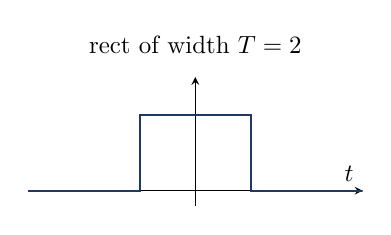
\begin{tikzpicture}[scale=0.9]
\begin{axis}[width=6.3cm,height=3.4cm,title={rect of width $T=2$},axis lines=middle,xlabel={$t$},ticks=none,ymax=1.5,ymin=-0.2,xmin=-3,xmax=3]\addplot[thick,navy,const plot]coordinates{(-3,0)(-1,0)(-1,1)(1,1)(1,0)(3,0)};\end{axis}
\end{tikzpicture}\hspace{4mm}
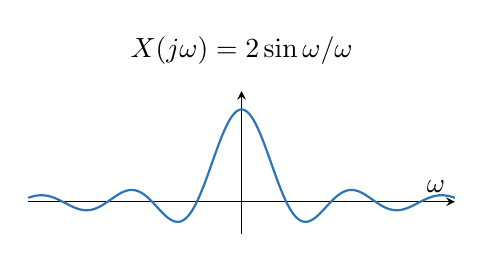
\begin{tikzpicture}
\begin{axis}[width=7cm,height=3.4cm,title={$X(j\omega)=2\sin\omega/\omega$},axis lines=middle,xlabel={$\omega$},ticks=none,samples=200,domain=-15:15,ymin=-0.7,ymax=2.4]\addplot[thick,sky]{2*sin(deg(x))/x};\end{axis}
\end{tikzpicture}\end{center}

\section{Properties}
\begin{formula}
\renewcommand{\arraystretch}{1.35}
\begin{tabular}{@{}lll@{}}
Time shift & $x(t-t_0)$ & $e^{-j\omega t_0}X$ (linear phase)\\
Frequency shift & $x(t)e^{j\omega_0t}$ & $X(j(\omega-\omega_0))$\\
Modulation & $x(t)\cos\omega_0t$ & $\tfrac12X(j(\omega-\omega_0))+\tfrac12X(j(\omega+\omega_0))$\\
Scaling & $x(at)$ & $\tfrac1{\abs a}X(j\omega/a)$\\
Reversal & $x(-t)$ & $X(-j\omega)$\\
Duality & $X(jt)$ & $2\pi x(-\omega)$\\
Differentiation & $\dfrac{\dd x}{\dd t}$ & $j\omega X$\\
Frequency differentiation & $-jt\,x(t)$ & $\dfrac{\dd X}{\dd\omega}$\\
Integration & $\int_{-\infty}^tx$ & $\dfrac{X}{j\omega}+\pi X(0)\delta(\omega)$\\
Convolution & $x*h$ & $XH$\\
Multiplication & $xy$ & $\tfrac1{2\pi}X*Y$\\
Real $x$ & & $\abs X$ even, $\angle X$ odd; even $x\Rightarrow X$ real
\end{tabular}
\end{formula}
\begin{proofbox}[Short proofs]
\emph{Shift:} $\int x(t-t_0)e^{-j\omega t}\dd t$, $\tau=t-t_0$ gives $e^{-j\omega t_0}X$. \emph{Frequency shift:} $\int xe^{j\omega_0t}e^{-j\omega t}\dd t=X(j(\omega-\omega_0))$. \emph{Convolution:} swap integrals, substitute $s=t-\tau$. \emph{Duality:} $2\pi x(-t)=\int Xe^{-j\omega t}\dd\omega$; rename $t\leftrightarrow\omega$.
\end{proofbox}
\begin{method}[Finding the FT of a given signal]
\begin{steps}
\item Match the signal (or pieces of it) to a table pair. \item Reduce the rest with shift, scaling, modulation, differentiation or reversal; \emph{name each property}. \item Decompose composite shapes into rectangles/triangles centred at their own centres and multiply each by $e^{-j\omega t_c}$. \item Sketch spectra: modulation gives two half-height copies at $\pm\omega_0$.
\end{steps}
\end{method}
\begin{example}{CSE 219 2022--23 Q6: $f=e^{-at}u(t)$, $\sgn t$}
$f(-t)=e^{at}u(-t)$. $F(j\omega)=\dfrac1{a+j\omega}$, $\F\{f(-t)\}=F(-j\omega)=\dfrac1{a-j\omega}$. $\sgn t=\lim_{a\to0}[f(t)-f(-t)]$, so by linearity and reversal
\[\F\{\sgn t\}=\lim_{a\to0}\left(\frac1{a+j\omega}-\frac1{a-j\omega}\right)=\frac{2}{j\omega}.\]
\end{example}
\begin{example}{CSE 219 2023--24 Q1(c): $\rect\!\left(\tfrac{t-\tau}T\right)\cos2\pi f_0t$}
$\rect(t)\leftrightarrow\sinc f=\frac{\sin\pi f}{\pi f}$; scaling: $\rect(t/T)\leftrightarrow T\sinc(fT)$; shift: $\times e^{-j2\pi f\tau}$; modulation:
\[X_2(f)=\tfrac T2\big[\sinc((f-f_0)T)e^{-j2\pi(f-f_0)\tau}+\sinc((f+f_0)T)e^{-j2\pi(f+f_0)\tau}\big].\]
\end{example}
\begin{example}{2023--24 Q2: $x_1=e^{-at}u$, $x_2=e^{-a\abs t}$ and $I(a)=\int\frac{f^2\dd f}{(a^2+(2\pi f)^2)^2}$}
$X_1=\frac1{a+j\omega}$; $x_2=x_1(t)+x_1(-t)\Rightarrow X_2=\frac{2a}{a^2+\omega^2}$. (The Parseval part $I(a)=\frac1{16\pi^2a}$ is outside Part-1 syllabus.)
\end{example}
\begin{example}{CSE 219 2022--23 Q5(b): inverse FT chain}
$X=1$ on $\abs\omega<3\pi$ gives $x(t)=\dfrac{\sin3\pi t}{\pi t}$. $X_1=3j\omega X$ (magnitude $3\abs\omega$, phase $\pm\frac\pi2$) so $x_1=3\dfrac{\dd x}{\dd t}=\dfrac{3(3\pi t\cos3\pi t-\sin3\pi t)}{\pi t^2}$.
\end{example}
\begin{inexam}
Spectrum sketches with modulation appear in every EEE paper (quadrature multiplexing 2023--24 Q5(a), AM with phase error: output $x(t)\cos\theta$). CSE 311: time delay $\Rightarrow$ linear phase, sampling spectra.
\end{inexam}

\section{Filters, distortionless systems, bandwidth}
\begin{formula}
$Y=HX$. Distortionless: $y=Kx(t-t_d)\Leftrightarrow H=Ke^{-j\omega t_d}$ ($\abs H$ constant, phase linear through the origin). All-pass: $\abs H$ constant but phase need not be linear. Ideal LPF with delay: $h=\dfrac{\sin\omega_c(t-t_d)}{\pi(t-t_d)}$ (non-causal, unrealizable). Compression in time $\Leftrightarrow$ expansion in frequency; derivative widens the spectrum. 3-dB bandwidth of $e^{-at}u$: $a$ rad/s.
\end{formula}
\begin{method}[Application sentences]
\textbf{Convolution}: reverb (convolve with the hall's impulse response), echo $h=\delta[n]+a\delta[n-D]$, smoothing (moving average). \textbf{Fourier series}: harmonic analysis, response to periodic sources. \textbf{Fourier transform}: denoising, JPEG (drop small high-frequency coefficients), MRI (data in frequency domain), music fingerprinting, vibration diagnosis, ECG notch.
\end{method}

\part{Ashraf Sir --- DFT, FFT and Sampling}

%=====================================================================
\chapter{DTFT, DFT and Circular Convolution}
%=====================================================================
\section{The four Fourier transforms and the DFT pair}
\begin{center}\small\begin{tabular}{@{}lll@{}}\toprule
 & continuous time & discrete time\\\midrule
periodic & CTFS: discrete, aperiodic $a_k$ & DFS/DFT: discrete, periodic $X[k]$\\
aperiodic & CTFT: continuous, aperiodic $X(j\omega)$ & DTFT: continuous, $2\pi$-periodic $X(e^{j\omega})$\\\bottomrule
\end{tabular}\end{center}
Rule: \emph{discrete in one domain $\Leftrightarrow$ periodic in the other.}
\begin{formula}
\begin{align*}
&W_N=e^{-j2\pi/N},\quad W_N^N=1,\quad W_N^{k+N/2}=-W_N^k,\\
&X[k]=\sum_{n=0}^{N-1}x[n]W_N^{kn},\qquad x[n]=\frac1N\sum_{k=0}^{N-1}X[k]W_N^{-kn},\\
&X(e^{j\omega})=\sum_nx[n]e^{-j\omega n}\ (2\pi\text{-periodic}),\qquad X[k]=X(e^{j\omega})\big|_{\omega=2\pi k/N},\\
&X[k]=Na_k\ (\text{DFS}),\qquad c_k=X[k]/T_0\ (\text{CTFS of the sampled signal}).
\end{align*}
Bins: $k=0..N/2$ positive frequencies (low$\to$high), $k=N/2..N-1$ negative (high$\to$low). $f_k=kf_s/N$ ($k\le N/2$), $(k-N)f_s/N$ above; resolution $\Delta f=f_s/N=1/T_0$.\\
Zero-padding to $M\ge N$: the same DTFT sampled every $2\pi/M$ (finer picture, no new information).
\end{formula}
\begin{center}\small
\begin{tabular}{@{}c|cccc|c@{}}
$W_4^{kn}$ & $n=0$ & 1 & 2 & 3 & \\\hline
$k=0$ & 1 & 1 & 1 & 1 & $W_4=-j$\\ $k=1$ & 1 & $-j$ & $-1$ & $j$ &\\ $k=2$ & 1 & $-1$ & 1 & $-1$ &\\ $k=3$ & 1 & $j$ & $-1$ & $-j$ &
\end{tabular}\qquad
\begin{tabular}{@{}c|cccc@{}}
$W_8^m$ & $m=0$ & 1 & 2 & 3\\\hline value & $1$ & $\tfrac{1-j}{\sqrt2}$ & $-j$ & $-\tfrac{1+j}{\sqrt2}$
\end{tabular}\end{center}
\begin{example}{$x=\{1,2,3,4\}$}
$X=\{10,\,-2+2j,\,-2,\,-2-2j\}$; check $X[0]=\sum x$, $X[3]=X^*[1]$; $\sum\abs x^2=30=\tfrac14(100+8+4+8)$.
\end{example}

\section{DFT properties}
\begin{formula}
\begin{tabular}{@{}lll@{}}
Circular shift & $x[((n-m))_N]$ & $W_N^{km}X[k]$\\
Modulation & $W_N^{-k_0n}x[n]$ & $X[((k-k_0))_N]$; $(-1)^nx\leftrightarrow X[k-N/2]$\\
Reversal / conjugation & $x[((-n))_N]$, $x^*[n]$ & $X[((-k))_N]$, $X^*[((-k))_N]$\\
Real $x$ & & $X[N-k]=X^*[k]$\\
Circular convolution & $x\circledast h$ & $X[k]H[k]$\\
Product & $x[n]h[n]$ & $\tfrac1NX\circledast H$\\
Parseval & $\sum\abs{x[n]}^2$ & $\tfrac1N\sum\abs{X[k]}^2$
\end{tabular}
\end{formula}

\section{Circular convolution and filtering with the DFT}
\begin{formula}
$(x\circledast h)[n]=\sum_{m=0}^{N-1}x[m]\,h[((n-m))_N]\ \Longleftrightarrow\ X[k]H[k]$. Linear convolution has length $L+M-1$; \textbf{circular $=$ linear iff $N\ge L+M-1$} (zero-pad both).
\end{formula}
\begin{method}[Linear convolution through the DFT]
\begin{steps}
\item Choose $N\ge L+M-1$ (power of 2 if an FFT is asked); zero-pad $x,h$.
\item Compute $X[k],H[k]$ (use the $W_N$ table).
\item $Y[k]=X[k]H[k]$ bin by bin.
\item $y[n]=\frac1N\sum Y[k]W_N^{-kn}$; check against the direct convolution.
\end{steps}
\end{method}
\begin{example}{CSE 219 2023--24 Q5(b): $\{1,2\}*\{1,1\}$ with $N=4$}
$X=\{3,\,1-2j,\,-1,\,1+2j\}$, $H=\{2,\,1-j,\,0,\,1+j\}$, $Y=\{6,\,-1-3j,\,0,\,-1+3j\}$. $y[n]=\tfrac14\sum Y[k]j^{kn}$ gives $y=\{1,3,2,0\}$.
\end{example}
\begin{example}{wrap-around}
$x=\{2,4,5,6,5,3,2,1\}$, $h=\{1,2,1\}$: linear $\{2,8,15,20,22,19,13,8,4,1\}$; circular ($N=8$) $\{6,9,15,20,22,19,13,8\}$ --- the tail $\{4,1\}$ folds onto the first two samples.
\end{example}

%=====================================================================
\chapter{Fast Fourier Transform}
%=====================================================================
\section{Radix-2 decimation in time (DIT)}
\begin{formula}
$X[k]=G[k]+W_N^kH[k]$, $X[k+\tfrac N2]=G[k]-W_N^kH[k]$ for $0\le k<\tfrac N2$, where $G,H$ are the $N/2$-point DFTs of the even and odd samples. Inputs in \textbf{bit-reversed} order, outputs natural.\\
Cost: direct $N^2$ multiplications vs FFT $\tfrac N2\log_2N$ (additions $N\log_2N$); $N=8$: $64$ vs $12$; $N=1024$: $1.05\times10^6$ vs $5120$.\\
Bit reversal, $N=8$: $x_0,x_4,x_2,x_6,x_1,x_5,x_3,x_7$.
\end{formula}
\begin{method}[Radix-2 DIT, every butterfly]
\begin{steps}
\item Zero-pad to $N=2^m$; write the bit-reversed input.
\item Stage 1: $(a,b)\mapsto(a+b,\,a-b)$ on adjacent pairs.
\item Stage 2: combine 2-point results with $W_4^0=1$, $W_4^1=-j$.
\item Stage 3: combine with $W_8^0\ldots W_8^3$: $X[k]=G[k]+W_8^kH[k]$, $X[k+4]=G[k]-W_8^kH[k]$.
\item Checks: $X[0]=\sum x$, $X[4]=\sum(-1)^nx[n]$, $X[8-k]=X^*[k]$.
\end{steps}
\end{method}
\begin{example}{CSE 219 2023--24 Q5(a): $x=\{1,2,3,4,3,2\}$, 8-point}
Pad: $\{1,2,3,4,3,2,0,0\}$; bit-reversed: $1,3,3,0,2,2,4,0$.\\
Stage 1: $4,-2\ |\ 3,3\ |\ 4,0\ |\ 4,4$.\\
Stage 2: $G=(7,\,-2-3j,\,1,\,-2+3j)$, $H=(8,\,-4j,\,0,\,4j)$.\\
Stage 3: $W_8^kH[k]=(8,\,-2.828-2.828j,\,0,\,2.828-2.828j)$.
\[X=\{15,\ -4.828-5.828j,\ 1,\ 0.828+0.172j,\ -1,\ 0.828-0.172j,\ 1,\ -4.828+5.828j\}.\]
\end{example}

\section{Decimation in frequency (DIF)}
\begin{formula}
$X[2m]=\mathrm{DFT}_{N/2}\{x[n]+x[n+\tfrac N2]\}$, $\;X[2m+1]=\mathrm{DFT}_{N/2}\{(x[n]-x[n+\tfrac N2])W_N^n\}$.\\
Butterfly: \emph{add/subtract first, then twiddle}. Inputs natural, outputs bit-reversed. Same cost as DIT.
\end{formula}

\section{Matrix (Cooley--Tukey / Bailey) FFT}
\begin{formula}
$N=N_1N_2$, $n=N_1n_2+n_1$ (column-major), $k=N_2k_1+k_2$ (row-major):
\[X[N_2k_1+k_2]=\sum_{n_1=0}^{N_1-1}W_N^{n_1k_2}\Big[\sum_{n_2=0}^{N_2-1}x[N_1n_2+n_1]W_{N_2}^{n_2k_2}\Big]W_{N_1}^{n_1k_1}.\]
\end{formula}
\begin{method}[Four-step FFT]
\begin{steps}
\item Arrange $x$ column-major in an $N_1\times N_2$ matrix (radix-2: row 0 = evens, row 1 = odds).
\item $N_2$-point DFT of every row $\to G$.
\item Multiply entry $(n_1,k_2)$ by $W_N^{n_1k_2}\to H$.
\item $N_1$-point DFT of every column; read the result \emph{row-major}.
\end{steps}
\end{method}
\begin{example}{CSE 219 2023--24 Q7(a): $x=\{1,2,3,4,9,0,7,8\}$}
Rows: $\{1,3,9,7\}$, $\{2,4,0,8\}$. $G=\begin{bmatrix}20&-8+4j&0&-8-4j\\14&2+4j&-10&2-4j\end{bmatrix}$. Twiddles of row 1: $1,\ 0.7071-0.7071j,\ -j,\ -0.7071-0.7071j$, so row 1 of $H$ is $14,\ 4.2426+1.4142j,\ 10j,\ -4.2426+1.4142j$. Column sums and differences give
\[X=\{34,\ -3.757+5.414j,\ 10j,\ -12.243-2.586j,\ 6,\ -12.243+2.586j,\ -10j,\ -3.757-5.414j\}.\]
\end{example}

\section{Fast convolution and Bluestein}
\begin{formula}
Fast convolution: pad to $N\ge L+M-1$, FFT both, multiply, IFFT: $O(N\log N)$ vs $O(LM)$.\\
Bluestein (any $N$, even prime): $kn=\tfrac12[n^2+k^2-(k-n)^2]$ gives
\[X[k]=W_{2N}^{k^2}\,(a*b)[k],\quad a[n]=x[n]W_{2N}^{n^2},\quad b[n]=W_{2N}^{-n^2},\ n=-(N-1)..(N-1),\]
$W_{2N}=e^{-j\pi/N}$. Pad to $M\ge2N-1$ (power of 2), with the negative-index chirp wrapped to the end so the two ends do not overlap.
\end{formula}
\begin{example}{3-point DFT of $\{2,-1,3\}$ by Bluestein}
$a=\{2,\,-0.5+0.866j,\,-1.5+2.598j\}$, $M=8$; result $X=\{4,\,1+3.464j,\,1-3.464j\}$, equal to the direct DFT.
\end{example}
\begin{inexam}
2023--24: Q5(a) 15 marks (8-point DIT), Q7(a) 15 (matrix FFT), Q7(b) 10 (Bluestein derivation); 2022--23 Q4(c) 15 (DFT vs FFT complexity: $N^2$ vs $\frac N2\log_2N$, speed-up $2N/\log_2N$).
\end{inexam}

%=====================================================================
\chapter{Sampling and Reconstruction}
%=====================================================================
\section{Spectrum of the sampled signal}
\begin{formula}
$x_p(t)=x(t)p(t)=\sum x(nT)\delta(t-nT)$, $\omega_s=2\pi/T$. $\;P(j\omega)=\dfrac{2\pi}T\sum_k\delta(\omega-k\omega_s)$ (impulse train $\to$ impulse train), and
\[\boxed{X_p(j\omega)=\frac1{2\pi}X*P=\frac1T\sum_{k=-\infty}^{\infty}X\big(j(\omega-k\omega_s)\big)}\]
Duality: $X(jt)\leftrightarrow2\pi x(-\omega)$; product $\leftrightarrow\frac1{2\pi}$ convolution. $\delta(\omega-k\omega_s)*X=X(j(\omega-k\omega_s))$.
\end{formula}
\begin{center}
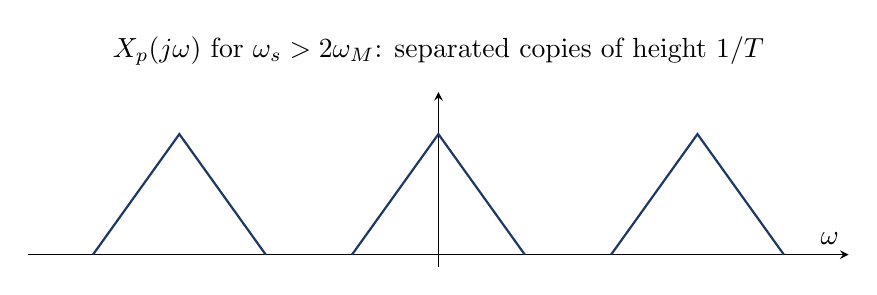
\begin{tikzpicture}
\begin{axis}[width=12cm,height=3.8cm,axis lines=middle,xlabel={$\omega$},ticks=none,ymin=-0.1,ymax=1.35,xmin=-9.5,xmax=9.5,title={$X_p(j\omega)$ for $\omega_s>2\omega_M$: separated copies of height $1/T$}]
\addplot[thick,navy,domain=-8:-4]{max(0,1-abs(x+6)/2)};
\addplot[thick,navy,domain=-2:2]{max(0,1-abs(x)/2)};
\addplot[thick,navy,domain=4:8]{max(0,1-abs(x-6)/2)};
\end{axis}
\end{tikzpicture}\end{center}

\section{Sampling theorem and aliasing}
\begin{formula}
Band-limited $X(j\omega)=0$ for $\abs\omega>\omega_M$ is uniquely determined by $x(nT)$ iff $\omega_s>2\omega_M$ (Nyquist rate $2\omega_M$; $T<\pi/\omega_M$). Product $xy$: bandwidths add. Aliasing: $f\to\abs{f-kf_s}$.\\
DT decimation: $X(e^{j\omega})=0$ for $W\le\abs\omega\le\pi$ allows keeping every $M$-th sample iff $M\le\pi/W$ (e.g.\ $W=2\pi/9\Rightarrow M=4$).
\end{formula}
\begin{proofbox}[Sampling theorem]
$X_p$ is $X/T$ repeated every $\omega_s$; copies of width $2\omega_M$ stay apart iff $\omega_M<\omega_s-\omega_M$, i.e.\ $\omega_s>2\omega_M$. Then an ideal LPF (gain $T$, $\omega_M<\omega_c<\omega_s-\omega_M$) isolates $X$. If $\omega_s<2\omega_M$ the copies overlap and add; the sum cannot be un-mixed, so $x$ is not recoverable.
\end{proofbox}
\begin{method}[Spectrum-sketch questions]
\begin{steps}
\item Sketch $X(j\omega)$; mark $\omega_M$. \item Compute $\omega_s=2\pi/T$ and compare with $2\omega_M$. \item Draw copies at $\pm k\omega_s$ with height $\times\frac1T$ (natural sampling: copies weighted by $c_k=\frac\tau T\sinc(\frac{k\tau}T)$). \item Overlap $\Rightarrow$ aliasing; cure: anti-aliasing LPF before sampling, higher rate, guard band.
\end{steps}
\end{method}
\begin{example}{EEE 301 2015-16 Q6(b): $z=xy$, 150 Hz and 350 Hz}
$z$ is band-limited to $500$ Hz, so $T_{s,\max}=1/(2\cdot500)=1$ ms. $T_s=0.5$ ms: copies every 2 kHz, no overlap; $T_s=2$ ms ($f_s=500$ Hz): copies of width 1 kHz overlap.
\end{example}
\begin{example}{EEE 211 2019--20 Q7(b)}
$x=\frac{\sin(\omega_Bt/2)}{\pi t}$ ($X=1$ on $\abs\omega<\omega_B/2$), $p=\sum\delta(t-n\pi/\omega_B)$ ($\omega_s=2\omega_B$). $Z=\frac{\omega_B}\pi\sum X(\omega-2k\omega_B)$; $h=\frac{\sin(3\omega_Bt/2)}{\pi t}$ passes $\abs\omega<1.5\omega_B$, i.e.\ only the centre copy: $y=\frac{\omega_B}\pi x(t)$.
\end{example}

\section{Reconstruction: sinc, zero-order hold, linear interpolation}
\begin{formula}
\renewcommand{\arraystretch}{1.4}
\begin{tabular}{@{}llll@{}}\toprule
 & $h(t)$ & $H(j\omega)$ & properties\\\midrule
Ideal & $\sinc(t/T)=\frac{\sin(\pi t/T)}{\pi t/T}$ & $T$ for $\abs\omega<\omega_s/2$ & non-causal, infinite\\
ZOH & rect on $[0,T]$ & $Te^{-j\omega T/2}\sinc\!\big(\frac{\omega T}{2\pi}\big)$ & causal; droop, leakage\\
Linear & triangle on $[-T,T]$ & $T\sinc^2\!\big(\frac{\omega T}{2\pi}\big)$ & non-causal; less leakage\\\bottomrule
\end{tabular}
\end{formula}
Ideal reconstruction: $x_r(t)=\sum x(nT)\sinc\!\big(\tfrac{t-nT}T\big)$. Triangle $=\frac1T\,h_0(t+\tfrac T2)*h_0(t+\tfrac T2)$. At $\omega_s/4$ ($T=1$): $\abs{H_0}=0.90$, $\abs{H_1}=0.81$.
\begin{inexam}
2023--24 Q5(c): which method for a real-time DAC with no non-causal filtering and no delay buffer? \mk{Zero-order hold}: causal, needs only the current sample; compensate the sinc droop with an analog low-pass.
\end{inexam}
\begin{example}{CSE 311 2018--19 Q1(a)}
Samples $g(0.01k)=\delta[k]$, $g$ band-limited to 50 Hz ($f_s=100$ Hz $=$ Nyquist): $g(t)=\dfrac{\sin100\pi t}{100\pi t}$, $G(f)=0.01\,\mathrm{rect}(f/100)$. As the band widens $g\to\delta(t)$ and $G\to1$.
\end{example}
\begin{pitfall}
Time-limited signals are never exactly band-limited, so some aliasing is unavoidable. For a periodic signal $X[k]=Na_k$ holds only if $a_k=0$ for $\abs k\ge N/2$.
\end{pitfall}

\part{Ashraf Sir --- Laplace and z-Transforms}

%=====================================================================
\chapter{The Laplace Transform}
%=====================================================================
\section{Definition, ROC and basic pairs}
\begin{formula}
\[X(s)=\int_{-\infty}^{\infty}x(t)e^{-st}\dd t=\F\{x(t)e^{-\sigma t}\},\quad s=\sigma+j\omega;\qquad x(t)=\frac1{2\pi j}\int_{\sigma-j\infty}^{\sigma+j\infty}X(s)e^{st}\dd s.\]
$s=j\omega$ gives the Fourier transform, valid only if the ROC contains the $j\omega$-axis. Eigenfunction: $e^{st}\to H(s)e^{st}$, $H=\Lap\{h\}$.\\
Unilateral (initial conditions at $0^-$): $\Lap\{y'\}=sY-y(0^-)$, $\Lap\{y''\}=s^2Y-sy(0^-)-y'(0^-)$.
\end{formula}
\begin{formula}[Pairs]
\renewcommand{\arraystretch}{1.35}
\begin{tabular}{@{}lll@{}}
$e^{-at}u(t)$ & $\dfrac1{s+a}$ & $\Re s>-a$\\
$-e^{-at}u(-t)$ & $\dfrac1{s+a}$ & $\Re s<-a$\\
$\delta(t)$ & $1$ & all $s$\\
$u(t)$ & $\dfrac1s$ & $\Re s>0$\\
$t^{n-1}e^{-at}u(t)/(n-1)!$ & $\dfrac1{(s+a)^n}$ & $\Re s>-a$\\
$e^{-at}\cos\omega_0t\,u(t)$ & $\dfrac{s+a}{(s+a)^2+\omega_0^2}$ & $\Re s>-a$\\
$e^{-at}\sin\omega_0t\,u(t)$ & $\dfrac{\omega_0}{(s+a)^2+\omega_0^2}$ & $\Re s>-a$\\
$e^{-b\abs t}$, $b>0$ & $\dfrac{-2b}{s^2-b^2}$ & $-b<\Re s<b$\\
$x=e^{-at}$ on $(0,T)$ & $\dfrac{1-e^{-(s+a)T}}{s+a}$ & all $s$ (no pole at $-a$)
\end{tabular}
\end{formula}
\begin{formula}[ROC rules]
(1) Vertical strips. (2) No poles inside. (3) Finite-duration absolutely integrable: entire plane. (4) Right-sided: $\Re s>\sigma_0$. (5) Left-sided: $\Re s<\sigma_0$. (6) Two-sided: a strip (or empty). (7--8) Rational: bounded by poles; right-sided $\Rightarrow$ right of the rightmost pole, left-sided $\Rightarrow$ left of the leftmost pole.
\end{formula}
\begin{center}
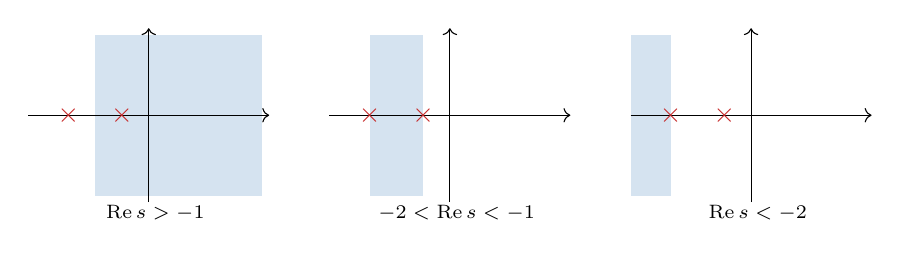
\begin{tikzpicture}[scale=0.85]
\begin{scope}[xshift=0cm]
\fill[sky!20] (0.8,-1.2) rectangle (3.3,1.2);\draw[->] (-0.2,0)--(3.4,0);\draw[->] (1.6,-1.3)--(1.6,1.3);
\node[crimson] at (0.4,0){$\times$};\node[crimson] at (1.2,0){$\times$};\node[below] at (1.7,-1.2){\scriptsize $\Re s>-1$};
\end{scope}
\begin{scope}[xshift=4.5cm]
\fill[sky!20] (0.4,-1.2) rectangle (1.2,1.2);\draw[->] (-0.2,0)--(3.4,0);\draw[->] (1.6,-1.3)--(1.6,1.3);
\node[crimson] at (0.4,0){$\times$};\node[crimson] at (1.2,0){$\times$};\node[below] at (1.7,-1.2){\scriptsize $-2<\Re s<-1$};
\end{scope}
\begin{scope}[xshift=9cm]
\fill[sky!20] (-0.2,-1.2) rectangle (0.4,1.2);\draw[->] (-0.2,0)--(3.4,0);\draw[->] (1.6,-1.3)--(1.6,1.3);
\node[crimson] at (0.4,0){$\times$};\node[crimson] at (1.2,0){$\times$};\node[below] at (1.7,-1.2){\scriptsize $\Re s<-2$};
\end{scope}
\end{tikzpicture}\\[-2pt]{\small Three ROCs of $X=\frac1{(s+1)(s+2)}$: three different signals.}
\end{center}
\begin{pitfall}
The expression alone does not give the signal --- always state the ROC. The ROC of a sum is the intersection of the ROCs (empty $\Rightarrow$ no transform). A time shift does not change the ROC; pole cancellation can enlarge it.
\end{pitfall}
\begin{method}[LT and ROC of a composite signal]
\begin{steps}
\item Split into right-sided, left-sided and finite pieces; transform each with its own ROC.
\item Use properties (shift $e^{-st_0}$, $s$-shift, $-tx\leftrightarrow X'(s)$, reversal $X(-s)$).
\item Intersect the ROCs; mark poles on the sketch.
\end{steps}
\end{method}
\begin{example}{CSE 219 2023--24 Q6(b)}
$x=\abs t\,e^{-2\abs t}-e^{-t}\cos3t\,u(t)+t^2e^{-4t}u(t)$.\\
$te^{-2t}u\leftrightarrow\frac1{(s+2)^2}$ ($\Re s>-2$); $(-t)e^{2t}u(-t)\leftrightarrow\frac{\dd}{\dd s}\!\big[\tfrac{-1}{s-2}\big]=\frac1{(s-2)^2}$ ($\Re s<2$); $e^{-t}\cos3t\,u\leftrightarrow\frac{s+1}{(s+1)^2+9}$ ($\Re s>-1$); $t^2e^{-4t}u\leftrightarrow\frac2{(s+4)^3}$ ($\Re s>-4$).
\[X(s)=\frac1{(s+2)^2}+\frac1{(s-2)^2}-\frac{s+1}{(s+1)^2+9}+\frac2{(s+4)^3},\qquad\boxed{-1<\Re s<2}.\]
Poles: $-2$ (double), $2$ (double), $-1\pm3j$, $-4$ (triple). The ROC contains the $j\omega$-axis.
\end{example}
\begin{example}{2022--23 Q1(b), Q2(c)}
$x=e^{-at}$ on $0<t<T$: $X=\frac{1-e^{-(s+a)T}}{s+a}$; at $s=-a$ the limit is $T$ (finite), so $s=-a$ \emph{is} in the ROC. $e^{-b\abs{t-2}}\leftrightarrow\dfrac{2be^{-2s}}{b^2-s^2}$, $-b<\Re s<b$.
\end{example}

\section{Properties}
\begin{formula}
\renewcommand{\arraystretch}{1.35}
\begin{tabular}{@{}llll@{}}
Linearity & $ax_1+bx_2$ & $aX_1+bX_2$ & $\supseteq R_1\cap R_2$\\
Time shift & $x(t-t_0)$ & $e^{-st_0}X$ & $R$\\
$s$-shift & $e^{s_0t}x(t)$ & $X(s-s_0)$ & $R+\Re s_0$\\
Scaling & $x(at)$ & $\frac1{\abs a}X(s/a)$ & $aR$\\
Reversal & $x(-t)$ & $X(-s)$ & $-R$\\
Convolution & $x_1*x_2$ & $X_1X_2$ & $\supseteq R_1\cap R_2$\\
Differentiation & $\dd x/\dd t$ & $sX$ & $\supseteq R$\\
$s$-differentiation & $-t\,x(t)$ & $\dd X/\dd s$ & $R$\\
Integration & $\int_{-\infty}^tx$ & $X/s$ & $\supseteq R\cap\{\Re s>0\}$
\end{tabular}\\[3pt]
Final value: if $sY(s)$ has all poles in the open LHP, $y(\infty)=\lim_{s\to0}sY(s)$. Initial value: $x(0^+)=\lim_{s\to\infty}sX(s)$.
\end{formula}
\begin{proofbox}[Differentiation]
$x=\frac1{2\pi j}\int Xe^{st}\dd s\Rightarrow x'=\frac1{2\pi j}\int sXe^{st}\dd s$, so $x'\leftrightarrow sX$ (e.g.\ $u\to\frac1s$, $\delta=u'\to1$: the pole cancels and the ROC grows). $s$-domain: $\frac{\dd X}{\dd s}=\int(-t)x(t)e^{-st}\dd t$. Final value: $\int_0^\infty y'e^{-st}\dd t=sY-y(0^-)\to y(\infty)-y(0^-)$ as $s\to0$.
\end{proofbox}

\section{Inverse Laplace transform}
\begin{method}[Partial fractions with the ROC]
\begin{steps}
\item If $\deg N\ge\deg D$ divide first (polynomial part $\to\delta,\delta'$).
\item Factor $D$; expand: simple pole $\frac A{s+a}$ with $A=(s+a)X\big|_{s=-a}$; repeated poles $\frac{A_1}{s+a}+\frac{A_2}{(s+a)^2}$; complex poles $\to$ complete the square ($e^{-\alpha t}\cos\beta t$, $e^{-\alpha t}\sin\beta t$).
\item Use the ROC: a pole to the \emph{left} of the ROC $\to$ right-sided term $Ae^{-at}u(t)$; a pole to the \emph{right} $\to$ left-sided term $-Ae^{-at}u(-t)$.
\item Check with $x(0^+)$ or one numeric value.
\end{steps}
\end{method}
\begin{example}{CSE 219 2022--23 Q2(b)}
$X=\dfrac{s+2}{s^2+7s+12}=\dfrac{-1}{s+3}+\dfrac2{s+4}$, ROC $-4<\Re s<-3$. Pole $-3$ is to the right of the ROC (left-sided), pole $-4$ to the left (right-sided):
\[x(t)=2e^{-4t}u(t)+e^{-3t}u(-t).\]
\end{example}
\begin{example}{several inversions}
$\frac{3s+7}{(s+1)(s+2)}=\frac4{s+1}-\frac1{s+2}\Rightarrow(4e^{-t}-e^{-2t})u$ ($\Re s>-1$). $\frac{-5}{(s+1)(s-4)}$, $-1<\Re s<4$: $e^{-t}u(t)+e^{4t}u(-t)$. $\frac{s}{s+2}=1-\frac2{s+2}\Rightarrow\delta-2e^{-2t}u$. $\frac{e^{-s}}{s(s+2)}\Rightarrow\tfrac12[1-e^{-2(t-1)}]u(t-1)$. $\frac1{(s-a)^3}\Rightarrow\tfrac12t^2e^{at}u$.
\end{example}

\section{LTI systems, differential equations, circuits, feedback}
\begin{formula}
$Y=HX$. DE $\sum a_ky^{(k)}=\sum b_kx^{(k)}$: $H(s)=\dfrac{\sum b_ks^k}{\sum a_ks^k}$ (zeros from the numerator, poles from the denominator); the equation does \emph{not} fix the ROC.\\
\textbf{Causal} $\Leftrightarrow$ ROC is a right half-plane. \textbf{Stable} $\Leftrightarrow$ ROC contains $j\omega$-axis; causal rational: all poles in the open LHP.\\
Cascade $H_1H_2$; parallel $H_1+H_2$; negative feedback $\dfrac{G}{1+GH}$; disturbance after controller: $H_d=\dfrac{G}{1+G_cG}$.
\end{formula}
\begin{method}[Solving a DE with initial conditions (unilateral)]
\begin{steps}
\item Transform: $Y\,D(s)=N(s)X(s)+I(s)$, with $I(s)=(s+a_1)y(0^-)+y'(0^-)$ for a second-order equation.
\item $\text{ZIR}=I/D$, $\text{ZSR}=NX/D$, $y=\text{ZIR}+\text{ZSR}$.
\item Partial fractions, invert, check $y(0^+)$.
\end{steps}
\end{method}
\begin{example}{CSE 219 2023--24 Q6(a)}
$y''+7y'+12y=x'+2x$, $x=u$, zero ICs: $Y=\dfrac{s+2}{s(s+3)(s+4)}=\dfrac{1/6}s+\dfrac{1/3}{s+3}-\dfrac{1/2}{s+4}$,
\[y(t)=\left[\tfrac16+\tfrac13e^{-3t}-\tfrac12e^{-4t}\right]u(t).\]
\end{example}
\begin{example}{EEE 211 2023--24 Q8(b)}
$y''+5y'+6y=x'+x$, $y(0^-)=2$, $y'(0^-)=1$, $x=e^{-4t}u$. ZIR: $\frac{2s+11}{(s+2)(s+3)}\Rightarrow7e^{-2t}-5e^{-3t}$. ZSR: $\frac{s+1}{(s+2)(s+3)(s+4)}\Rightarrow-\tfrac12e^{-2t}+2e^{-3t}-\tfrac32e^{-4t}$.
\[y=(6.5e^{-2t}-3e^{-3t}-1.5e^{-4t})u(t),\quad y(0^+)=2\ \checkmark.\]
\end{example}
\begin{example}{CSE 219 2023--24 Q6(c): ROC reasoning}
Causal but unstable: $H=\frac1{s-2}$, ROC $\Re s>2$ (right half-plane $\Rightarrow$ causal; pole in RHP so the ROC excludes $j\omega$). Stable but non-causal: $H=\frac{-2}{s^2-1}$, ROC $-1<\Re s<1$, $h=e^{-\abs t}$. For $H=\frac{s-1}{(s+1)(s-2)}$: $\Re s>2$ causal--unstable; $-1<\Re s<2$ stable--non-causal; $\Re s<-1$ anti-causal--unstable.
\end{example}
\begin{method}[Circuits]
\begin{steps}
\item Initial states: $v_C(0^-)$, $i_L(0^-)$ (for a source that is on at $t<0$, use the dc steady state at $0^-$).
\item s-domain models: $R$; $L\to sL$ in series with $Li_L(0^-)$ (or parallel with $i_L(0^-)/s$); $C\to\frac1{sC}$ in series with $\frac{v_C(0^-)}s$.
\item KVL/KCL or division; partial fractions; invert; check $y(0^+)$.
\end{steps}
\end{method}
\begin{example}{EEE 211 2023--24 Q4(a): series $L=2$\,H, then $R=1\,\Omega\parallel C=2$\,F, $y=v_C$}
$v_C(0^-)=1$, $i_L(0^-)=2$, $x=u$: $\frac1s=2(sI-2)+V$, $I=(2s+1)V-2\Rightarrow V(4s^2+2s+1)=\frac1s+4s+4$.
\[Y=\frac1s+\frac2{4s^2+2s+1},\qquad y(t)=\left[1+\tfrac2{\sqrt3}e^{-t/4}\sin\tfrac{\sqrt3t}4\right]u(t).\]
\end{example}
\begin{example}{EEE 211 2023--24 Q5(b): steady-state with a controller}
Unity feedback, plant $\frac1{s+2}$, $G_c=\frac{s+1}s$: $T=\frac{s+1}{s^2+3s+1}$, poles stable, $T(0)=1$ so $y(\infty)=A$ (integral action). With $G_c=\frac1{s-2}$: $T=\frac1{s^2-3}$ has a pole at $+\sqrt3$: unstable, the final-value theorem does not apply.
\end{example}
\begin{example}{other recurring checks}
$y''+4y'+3y=u$, $y(0^-)=2$, $y'(0^-)=1$: $y=\tfrac13+3e^{-t}-\tfrac43e^{-3t}$. $y''+5y'+6y=2e^{-t}u$, $y(0^-)=3$, $y'(0^-)=-2$: $y=e^{-t}+5e^{-2t}-3e^{-3t}$. $H=\frac{s^2+5s+5}{s^2+5s+6}$: $h=\delta+(e^{-3t}-e^{-2t})u$. $H=\frac{2s+1}{(s+1)(s+2)}$: $h=(3e^{-2t}-e^{-t})u$. Closed loop with $H_1=\frac1{s^2+bs+b-3}$, $H_2=-2$: $H=\frac1{s^2+bs+b-5}$, stable for $b>5$.
\end{example}
\begin{inexam}
EEE papers: 2--3 Laplace questions every year (DE with ICs, RLC circuit, block diagram/feedback, final value). CSE 219: 2022--23 Q1--Q2 (32 marks), 2023--24 Q6 (35 marks). Figure-based questions: write $H(s)$ from the diagram first.
\end{inexam}

%=====================================================================
\chapter{The $z$-Transform}
%=====================================================================
\section{Definition, ROC and pairs}
\begin{formula}
\[X(z)=\sum_{n=-\infty}^{\infty}x[n]z^{-n},\quad z=re^{j\omega},\quad X(re^{j\omega})=\F\{x[n]r^{-n}\},\quad z=e^{sT}.\]
The DTFT exists iff the ROC contains $\abs z=1$. $y[n]=H(z)z^n$ for input $z^n$.
\end{formula}
\begin{formula}[Pairs]
\renewcommand{\arraystretch}{1.35}
\begin{tabular}{@{}lll@{}}
$a^nu[n]$ & $\dfrac1{1-az^{-1}}$ & $\abs z>\abs a$\\
$-a^nu[-n-1]$ & $\dfrac1{1-az^{-1}}$ & $\abs z<\abs a$\\
$\delta[n],\ \delta[n-1],\ \delta[n+1]$ & $1,\ z^{-1},\ z$ & all $z$; $z\ne0$; finite $z$\\
$a^n$, $0\le n\le N-1$ & $\dfrac{1-a^Nz^{-N}}{1-az^{-1}}$ & $z\ne0$\\
$na^nu[n]$ & $\dfrac{az^{-1}}{(1-az^{-1})^2}$ & $\abs z>\abs a$\\
$b^{\abs n}$, $0<b<1$ & $\dfrac{1-b^2}{(1-bz^{-1})(1-bz)}$ & $b<\abs z<1/b$\\
$(\tfrac13)^n\sin(\tfrac\pi4n)u[n]$ & $\dfrac{\frac{\sqrt2}6z^{-1}}{1-\frac{\sqrt2}3z^{-1}+\frac19z^{-2}}$ & $\abs z>\frac13$
\end{tabular}
\end{formula}
\begin{formula}[ROC rules]
Ring centred at the origin; no poles inside; finite sequence: all $z$ except $0$ (terms with $n>0$) and/or $\infty$ (terms with $n<0$); right-sided $\Rightarrow$ exterior of a circle (includes $\infty$ iff causal); left-sided $\Rightarrow$ interior; two-sided $\Rightarrow$ annulus. Rational: right-sided outside the outermost pole, left-sided inside the innermost pole.
\end{formula}
\begin{center}
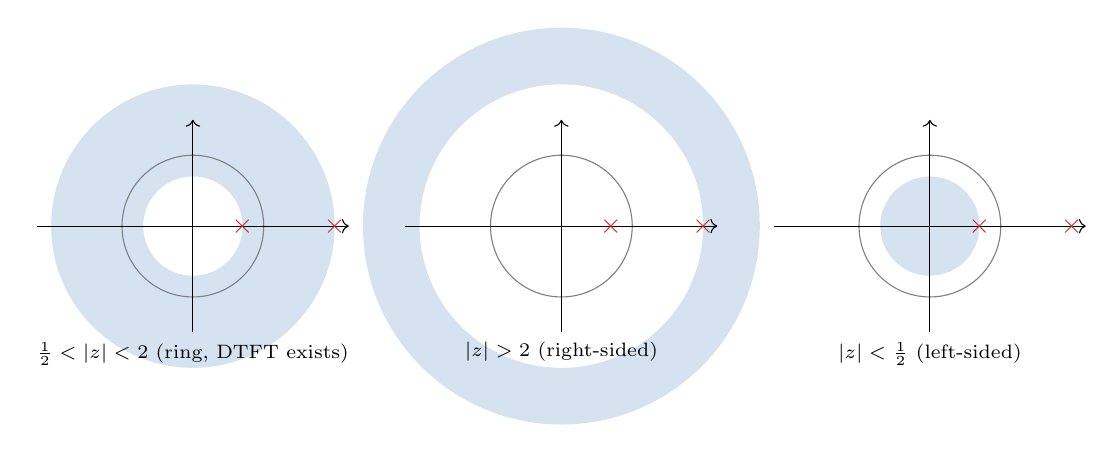
\begin{tikzpicture}[scale=0.9]
\foreach \xs/\ra/\rb/\tt in {0/0.7/2.0/{$\tfrac12<\abs z<2$ (ring, DTFT exists)},5.2/2.0/2.8/{$\abs z>2$ (right-sided)},10.4/0/0.7/{$\abs z<\tfrac12$ (left-sided)}}{
\begin{scope}[xshift=\xs cm]
\fill[sky!20] (0,0) circle (\rb);\ifdim\ra cm>0cm\fill[white] (0,0) circle (\ra);\fi
\draw[gray] (0,0) circle (1.0);\draw[->] (-2.2,0)--(2.2,0);\draw[->] (0,-1.5)--(0,1.5);
\node[crimson] at (0.7,0){$\times$};\node[crimson] at (2.0,0){$\times$};
\node[below] at (0,-1.5){\scriptsize \tt};
\end{scope}}
\end{tikzpicture}\\[-2pt]{\small Poles at $\tfrac12$ and $2$; only the ring contains the unit circle (grey).}
\end{center}
\begin{example}{CSE 219 2022--23 Q1(a), Q3(a)}
$\sum_{n\ge0}a^nz^{-n}=\frac1{1-az^{-1}}$ for $\abs{az^{-1}}<1\Leftrightarrow\abs z>\abs a$. For $x[n]=a^n$, $0\le n\le N-1$, $X(z)$ contains $az^{-1}\to\infty$ as $z\to0$, so $0\notin\ROC$; ROC is $\abs z>0$ (closed form $\frac{z(1-a^Nz^{-N})}{z-a}$ has $N-1$ poles at the origin; the pole at $a$ cancels).
\end{example}

\section{Inverse $z$-transform}
\begin{formula}
Contour: $x[n]=\dfrac1{2\pi j}\oint_CX(z)z^{n-1}\dd z$ ($C$ in the ROC, counter-clockwise). Derivation: inverse DTFT of $X(re^{j\omega})r^{-n}$, then $\dd z=jz\dd\omega$.
\end{formula}
\begin{method}[Inversion]
\begin{steps}
\item Write $X$ in powers of $z^{-1}$ with unit constant terms; expand in partial fractions $\frac A{1-pz^{-1}}$.
\item $\abs p<$ inner edge of the ROC (pole inside) $\to Ap^nu[n]$; pole outside the ROC $\to -Ap^nu[-n-1]$.
\item Irrational $X$ (log): expand in a power series of $z^{-1}$ valid in the ROC and read $x[n]$ as the coefficient of $z^{-n}$.
\item Causal check: $x[0]=\lim_{z\to\infty}X(z)$.
\end{steps}
\end{method}
\begin{example}{CSE 219 2022--23 Q3(c): $X=\log(1+az^{-1})$, $\abs z>\abs a$}
$\log(1+v)=\sum_{n\ge1}(-1)^{n+1}\frac{v^n}n$ for $\abs v<1$; $v=az^{-1}$ satisfies this exactly for $\abs z>\abs a$:
\[x[n]=(-1)^{n+1}\frac{a^n}{n}\,u[n-1].\]
\end{example}
\begin{example}{CSE 219 2023--24 Q8(a)}
$X=\dfrac{1+2z^{-1}-z^{-2}}{1-\frac{11}6z^{-1}+z^{-2}-\frac16z^{-3}}=\dfrac6{1-z^{-1}}-\dfrac3{1-\frac12z^{-1}}-\dfrac2{1-\frac13z^{-1}}$, poles $1,\tfrac12,\tfrac13$.\\
$\abs z>1$: $x=[6-3(\tfrac12)^n-2(\tfrac13)^n]u[n]$.\\
$\tfrac12<\abs z<1$: $x=-6u[-n-1]-3(\tfrac12)^nu[n]-2(\tfrac13)^nu[n]$.\\
$\tfrac13<\abs z<\tfrac12$: $x=-6u[-n-1]+3(\tfrac12)^nu[-n-1]-2(\tfrac13)^nu[n]$.\\
$\abs z<\tfrac13$: $x=-6u[-n-1]+3(\tfrac12)^nu[-n-1]+2(\tfrac13)^nu[-n-1]$.\\
The pole at $z=1$ lies on the unit circle: no ROC contains it, so no DTFT exists.
\end{example}

\section{Properties and LTI systems}
\begin{formula}
\renewcommand{\arraystretch}{1.35}
\begin{tabular}{@{}llll@{}}
Time shift & $x[n-n_0]$ & $z^{-n_0}X$ & $R$ (except $0,\infty$)\\
$z$-scaling & $a_0^nx[n]$ & $X(z/a_0)$ & $\abs{a_0}R$\\
Reversal & $x[-n]$ & $X(z^{-1})$ & $R^{-1}$\\
Expansion & $x[n/k]$ & $X(z^k)$ & $R^{1/k}$\\
Convolution & $x*h$ & $XH$ & $\supseteq R_1\cap R_2$\\
First difference & $x[n]-x[n-1]$ & $(1-z^{-1})X$ & \\
Accumulation & $\sum_{k\le n}x[k]$ & $\frac{X}{1-z^{-1}}$ & $\supseteq R\cap\abs z>1$\\
$z$-differentiation & $nx[n]$ & $-z\frac{\dd X}{\dd z}$ & $R$\\
Initial value & $x[0]$ (causal) & $\lim_{z\to\infty}X$ &
\end{tabular}\\[3pt]
\textbf{Causal} $\Leftrightarrow$ ROC is an exterior including $\infty$. \textbf{Stable} $\Leftrightarrow$ ROC contains the unit circle. Causal rational: stable iff all poles inside $\abs z=1$. Difference equation: $H=\dfrac{\sum b_kz^{-k}}{\sum a_kz^{-k}}$, ROC from causality.
\end{formula}
\begin{example}{Difference equation}
$y[n]-\tfrac12y[n-1]=x[n]+\tfrac13x[n-1]$: $H=\frac{1+\frac13z^{-1}}{1-\frac12z^{-1}}$, ROC $\abs z>\tfrac12$ (causal). Step response: $Y=\frac{8/3}{1-z^{-1}}-\frac{5/3}{1-\frac12z^{-1}}$, $y[n]=\tfrac83u[n]-\tfrac53(\tfrac12)^nu[n]$.
\end{example}
\begin{example}{CSE 219 2023--24 Q8(b): pole--zero reasoning (poles $\tfrac13,\tfrac23,2$)}
\begin{center}\small\begin{tabular}{@{}ll@{}}\toprule
statement & ROC\\\midrule
right-sided & $\abs z>2$\\ FT converges & $\tfrac23<\abs z<2$\\ FT does not converge & $\abs z>2$, or $\tfrac13<\abs z<\tfrac23$, or $\abs z<\tfrac13$\\ left-sided & $\abs z<\tfrac13$\\\bottomrule
\end{tabular}\end{center}
\end{example}
\begin{example}{CSE 219 2023--24 Q8(c): $x[n]=\abs n(\tfrac12)^{\abs n}$}
$n\ge0$: $n(\tfrac12)^nu[n]\leftrightarrow\frac{\frac12z^{-1}}{(1-\frac12z^{-1})^2}$, $\abs z>\tfrac12$. $n<0$: with $m=-n$, $\sum m(\tfrac12)^mz^m=\frac{\frac12z}{(1-\frac12z)^2}$, $\abs z<2$.
\[X(z)=\frac{2z(5z^2-8z+5)}{(z-2)^2(2z-1)^2},\quad\tfrac12<\abs z<2.\]
Poles: $\tfrac12$ (double), $2$ (double); zeros: $0$ and $0.8\pm0.6j$ (on the unit circle). Check $X(1)=4=\sum\abs n(\tfrac12)^{\abs n}$.
\end{example}
\begin{example}{CSE 219 2023--24 Q8(d): Laplace vs $z$}
$\Lap$: continuous time, $s=\sigma+j\omega$, strips/half-planes, stability: ROC contains $j\omega$. $\Z$: discrete time, $z=re^{j\omega}$, rings, stability: ROC contains $\abs z=1$; $z=e^{sT}$. The map $s\to e^{sT}$ is many-to-one (s and $s+j2\pi/T$ give the same sequence), so $z$ removes that redundancy and turns difference equations into algebra.
\end{example}

\appendix
\chapter{Question-Type Map and Exam Checklist}
\section{Which method for which question (recent papers)}
\begin{center}\small\renewcommand{\arraystretch}{1.3}
\begin{tabularx}{\textwidth}{@{}>{\raggedright\arraybackslash}p{4.2cm}X>{\raggedright\arraybackslash}p{3.1cm}@{}}\toprule
\textbf{Question type} & \textbf{Go to} & \textbf{Recent TF}\\midrule
Sketch $x(\alpha t+\beta)$, sums of shifted/scaled pieces & Ch.\,1 \S1.2 recipe, $t=(a-\beta)/\alpha$ & 22-23 Q7; 23-24 Q1(a)\\
Even--odd decomposition + graphs & Ch.\,1 \S1.3 & 22-23 Q5(a)\\
Periodicity (DT/CT) & Ch.\,1 \S1.5 & 22-23 Q5(c); 23-24 Q3(a)\\
System properties, interconnections, $h_{eq}$ & Ch.\,2 \S2.1--2.2 & 23-24 Q1(b)\\
DT/CT convolution, interval table & Ch.\,2 \S2.3 & 22-23 Q8(a)\\
Causal? stable? & Ch.\,2 \S2.4 & 22-23 Q8(b); 23-24 Q3(b)\\
FS coefficients, shift/derivative properties & Ch.\,3 & 23-24 Q4\\
FT of a signal with properties, spectra & Ch.\,4 & 22-23 Q5(b), Q6; 23-24 Q1(c), Q2\\
8-pt DIT FFT, matrix FFT, Bluestein & Ch.\,6 & 23-24 Q5(a), Q7(a),(b)\\
Linear convolution via DFT & Ch.\,5 & 23-24 Q5(b)\\
Sampling theorem, aliasing, reconstruction & Ch.\,7 & 22-23 Q1(c), Q4(b); 23-24 Q5(c), Q7(c)\\
LT + ROC, inverse LT, properties & Ch.\,8 & 22-23 Q1(b), Q2; 23-24 Q6\\
$z$-transform, ROC, inverse & Ch.\,9 & 22-23 Q1(a), Q3; 23-24 Q8\\\bottomrule
\end{tabularx}\end{center}

\section{Universal exam checklist}
\begin{method}[Before you write]
\begin{steps}
\item Read the whole question; underline what is asked (draw, prove, state the ROC, name the property).
\item Sketch first --- signals, overlap, spectra, ROC strips and pole--zero plots.
\item Write steps in your own compact way; show intermediate signals/matrices when the question says ``showing all stages''.
\item Check at the end: units/limits, continuity at interval boundaries, $X[0]=\sum x$, $y(0^+)$, support, stability of poles.
\item Always state the ROC next to every Laplace and $z$ answer.
\end{steps}
\end{method}
\begin{pitfall}[Frequent mistakes]
\begin{itemize}[leftmargin=1.4em,itemsep=1pt]
\item Order of shift and scaling; forgetting the reversal when $\alpha<0$.
\item Dropping the $n<0$ (or $t<0$) region of a convolution.
\item Impulses at jumps lost when differentiating.
\item $a_0$ missing after integrating or dividing by $jk\omega_0$.
\item Wrong twiddle: $W_8^3=-\frac{1+j}{\sqrt2}$, $W_4=-j$ (not $+j$).
\item Giving a Laplace/$z$ expression without the ROC; picking the wrong-sided term for a pole.
\item Using the final-value theorem when poles lie in the right half-plane or on the $j\omega$-axis.
\end{itemize}
\end{pitfall}
\end{document}

